\documentclass[10pt, a4paper]{article}
\usepackage[margin=1.5cm]{geometry}
\usepackage{graphicx}
\usepackage{booktabs}
\usepackage{subcaption}
\usepackage{float}
\usepackage{amsmath}
\usepackage{mathpazo}
\usepackage[utf8]{inputenc}
\usepackage[T2A]{fontenc}
\usepackage[english,russian]{babel}

\title{Polarimetric Analysis of Dust Continuum in Molecular Clouds}
\author{BISTRO Data Pipeline}
\date{\today}

\begin{document}

\maketitle

\section*{Methodology and Processing Parameters}

This report presents the automated polarimetric analysis of dust continuum emission. The pipeline abandons arbitrary geometric cropping in favor of rigorous statistical isolation of dense molecular clumps.

\paragraph{Statistical Segmentation and Masking:}
To mitigate edge artifacts, a geometric safety margin is established via distance transform. Within this zone, physical structures are isolated using a dynamic threshold based on the local median and standard deviation of Stokes $I$ ($I > \tilde{I} + N\sigma_I$). Morphological dilation ensures the preservation of compact cores and the continuity of diffuse filaments. The background is strictly masked (assigned \texttt{NaN}), ensuring that polarization parameters and subsequent statistics are calculated exclusively within the identified physical structures.

\paragraph{Plot Structure:}
For each targeted region, the analysis yields three diagnostic panels:
\begin{enumerate}
    \item \textbf{Statistical Segmentation (Top Left):} Isophotes and morphological boundaries of the isolated dense cores over the asinh-stretched Stokes $I$ continuum.
    \item \textbf{SNR-Coded Magnetic Field (Top Right):} Polarization vectors ($E$-field rotated by 90$^\circ$) overlaid on the full continuum map. Vectors are strictly constrained to the segmented areas and color-coded by the polarized intensity signal-to-noise ratio ($\text{SNR}_{pI}$).
    \item \textbf{Structure Function (Bottom Center):} Angular dispersion of the magnetic field $D_\phi(R)$ plotted against the spatial lag $R$ (in parsecs), calculated strictly within the isolated clumps.
\end{enumerate}

\newpage
\section*{Target: Auriga}

\begin{table}[H]
    \centering
    \renewcommand{\arraystretch}{1.1}
    \begin{tabular}{ll}
        \toprule
        \textbf{Parameter} & \textbf{Value} \\
        \midrule
        Distance (pc) & 450.0 \\
        Effective Pixels & 4012 \\
        Stokes I RMS & 42.87812 \\
        Median SNR & 1.36 \\
        Distance Reference & Lada et al. 2009 \\
        Vector Decimation Step & 4 px \\
        \bottomrule
    \end{tabular}
\end{table}

\vspace{0.5cm}

\begin{figure}[H]
    \centering
    \begin{subfigure}{0.48\textwidth}
        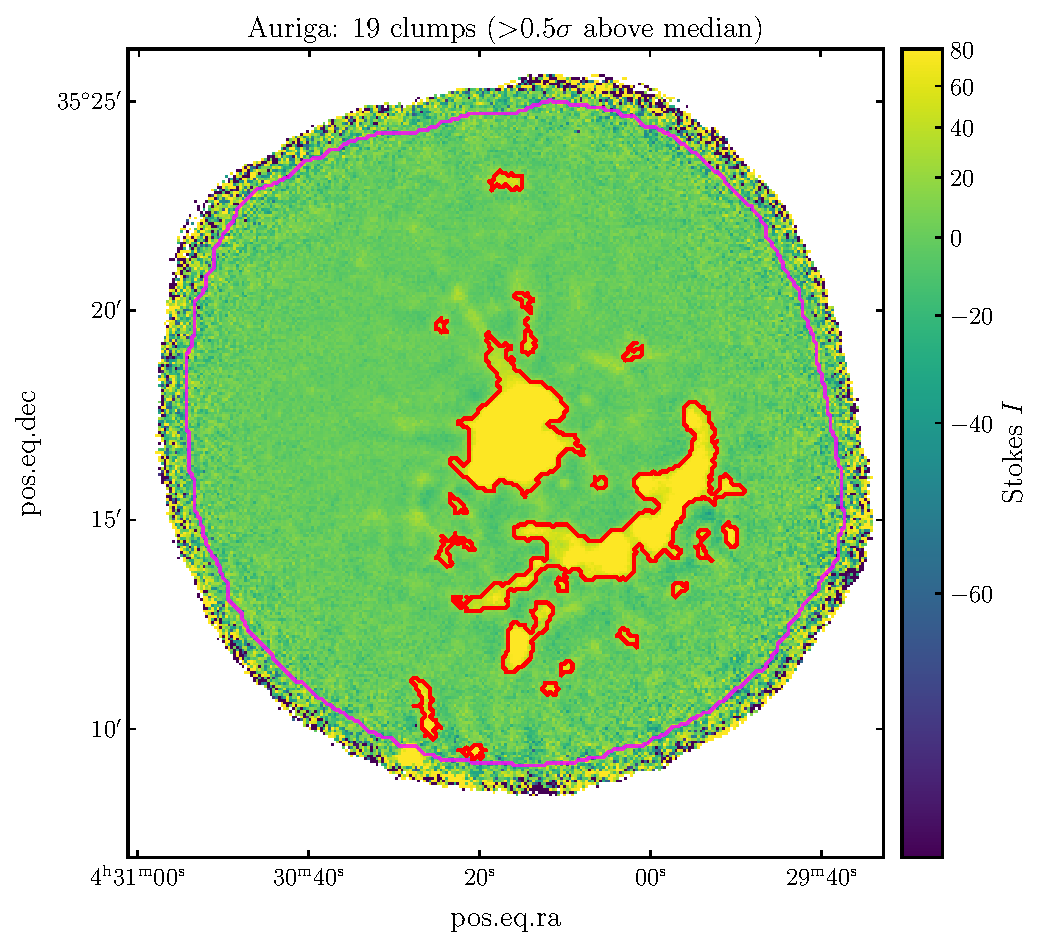
\includegraphics[width=\linewidth]{../plots/Auriga/Auriga_stat_segmentation.pdf}
    \end{subfigure}
    \hfill
    \begin{subfigure}{0.48\textwidth}
        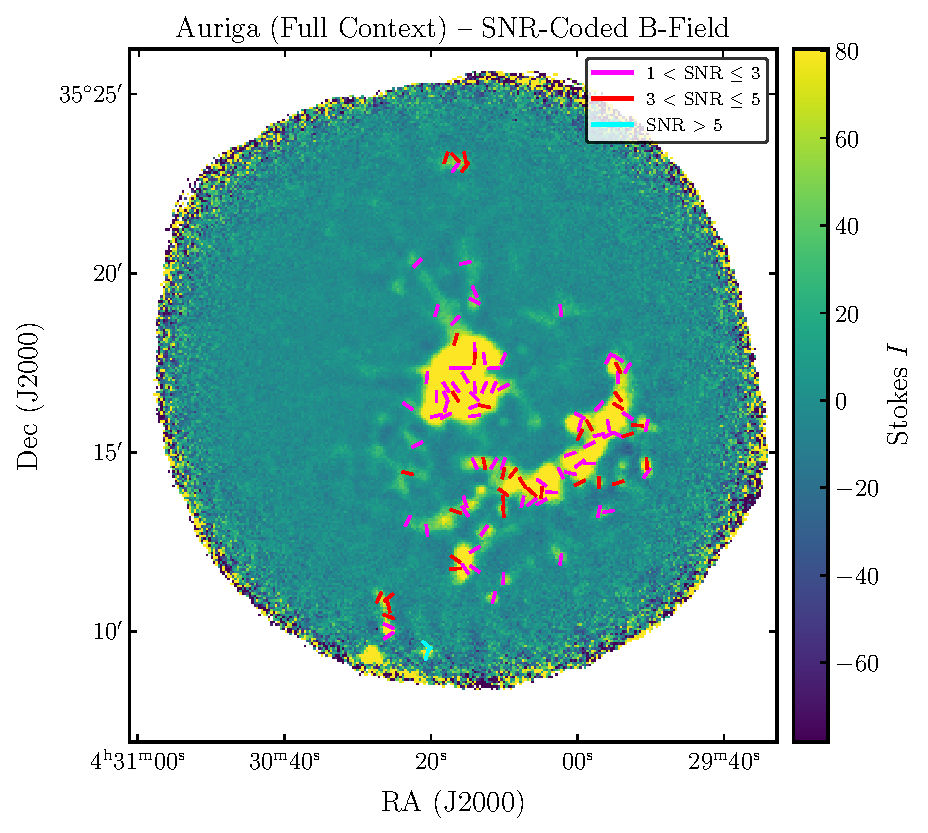
\includegraphics[width=\linewidth]{../plots/Auriga/Auriga_snr_colored_full.pdf}
    \end{subfigure}
    
    \vspace{0.5cm}
    
    \begin{subfigure}{0.6\textwidth}
        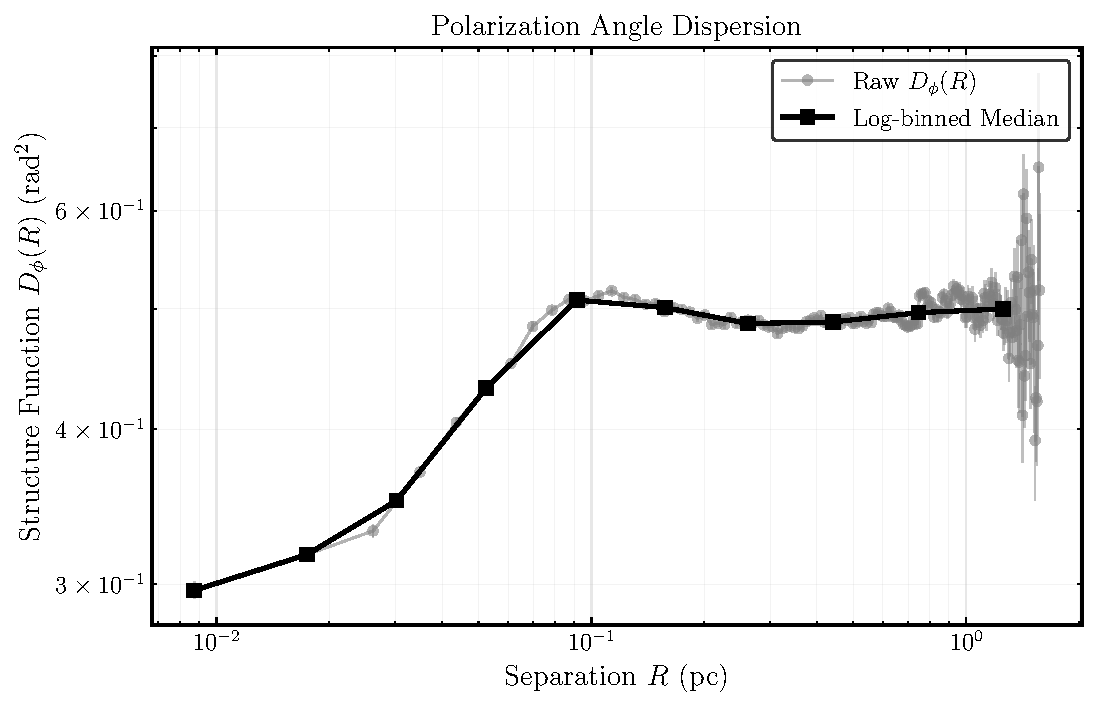
\includegraphics[width=\linewidth]{../plots/Auriga/Auriga_sf.pdf}
    \end{subfigure}
\end{figure}

\newpage
\section*{Target: L1495}

\begin{table}[H]
    \centering
    \renewcommand{\arraystretch}{1.1}
    \begin{tabular}{ll}
        \toprule
        \textbf{Parameter} & \textbf{Value} \\
        \midrule
        Distance (pc) & 140.0 \\
        Effective Pixels & 953 \\
        Stokes I RMS & 7.25939 \\
        Median SNR & 1.46 \\
        Distance Reference & Galli et al. 2018 / Schlafly et al. 2014 \\
        Vector Decimation Step & 2 px \\
        \bottomrule
    \end{tabular}
\end{table}

\vspace{0.5cm}

\begin{figure}[H]
    \centering
    \begin{subfigure}{0.48\textwidth}
        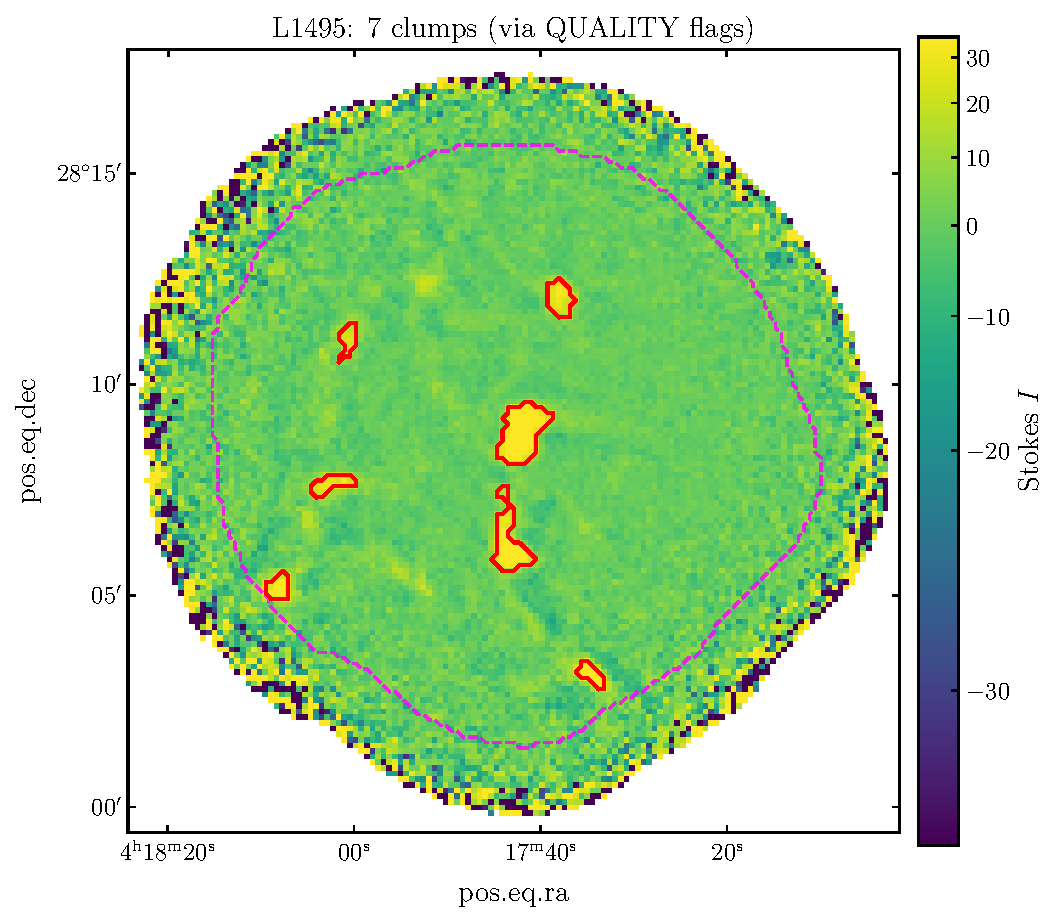
\includegraphics[width=\linewidth]{../plots/L1495/L1495_stat_segmentation.pdf}
    \end{subfigure}
    \hfill
    \begin{subfigure}{0.48\textwidth}
        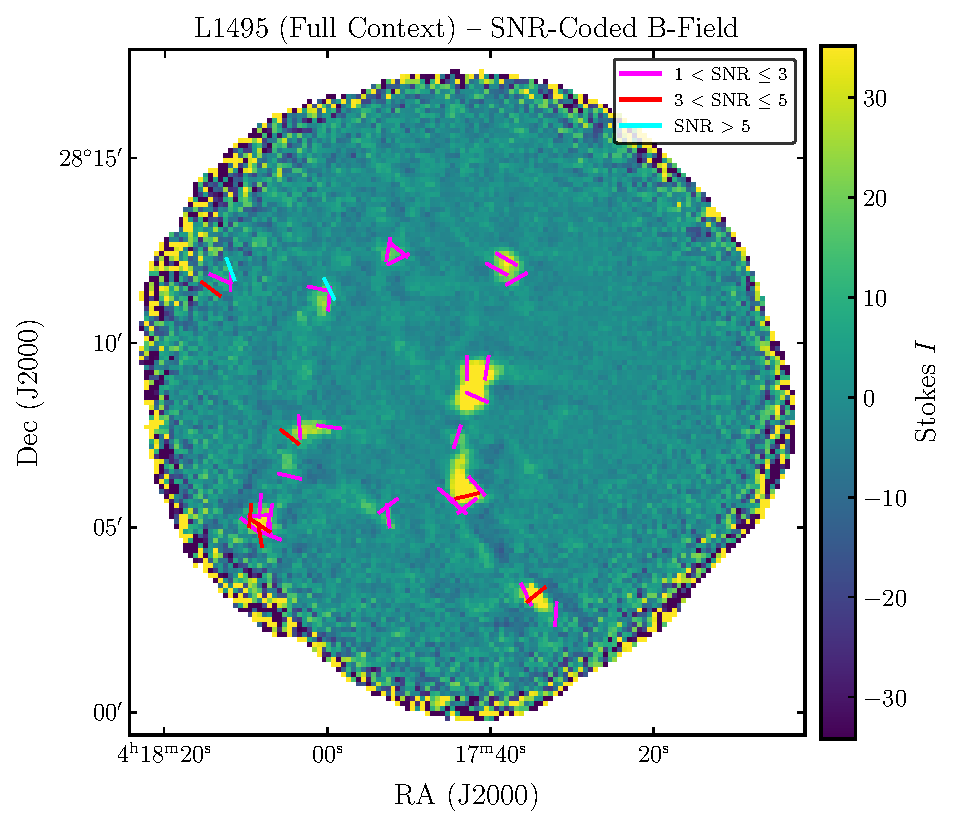
\includegraphics[width=\linewidth]{../plots/L1495/L1495_snr_colored_full.pdf}
    \end{subfigure}
    
    \vspace{0.5cm}
    
    \begin{subfigure}{0.6\textwidth}
        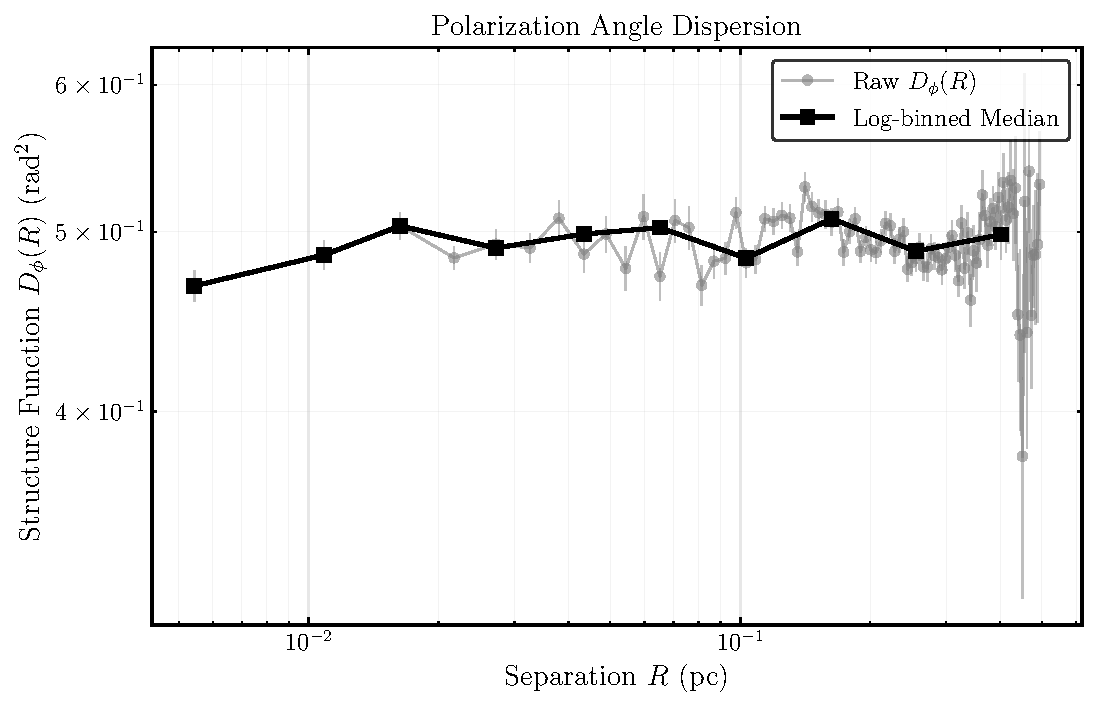
\includegraphics[width=\linewidth]{../plots/L1495/L1495_sf.pdf}
    \end{subfigure}
\end{figure}

\newpage
\section*{Target: L43\_Karoly\_2023}

\begin{table}[H]
    \centering
    \renewcommand{\arraystretch}{1.1}
    \begin{tabular}{ll}
        \toprule
        \textbf{Parameter} & \textbf{Value} \\
        \midrule
        Distance (pc) & 125.0 \\
        Effective Pixels & 439 \\
        Stokes I RMS & 48.02407 \\
        Median SNR & 1.10 \\
        Distance Reference & Ortiz-León et al. 2017 \\
        Vector Decimation Step & 2 px \\
        \bottomrule
    \end{tabular}
\end{table}

\vspace{0.5cm}

\begin{figure}[H]
    \centering
    \begin{subfigure}{0.48\textwidth}
        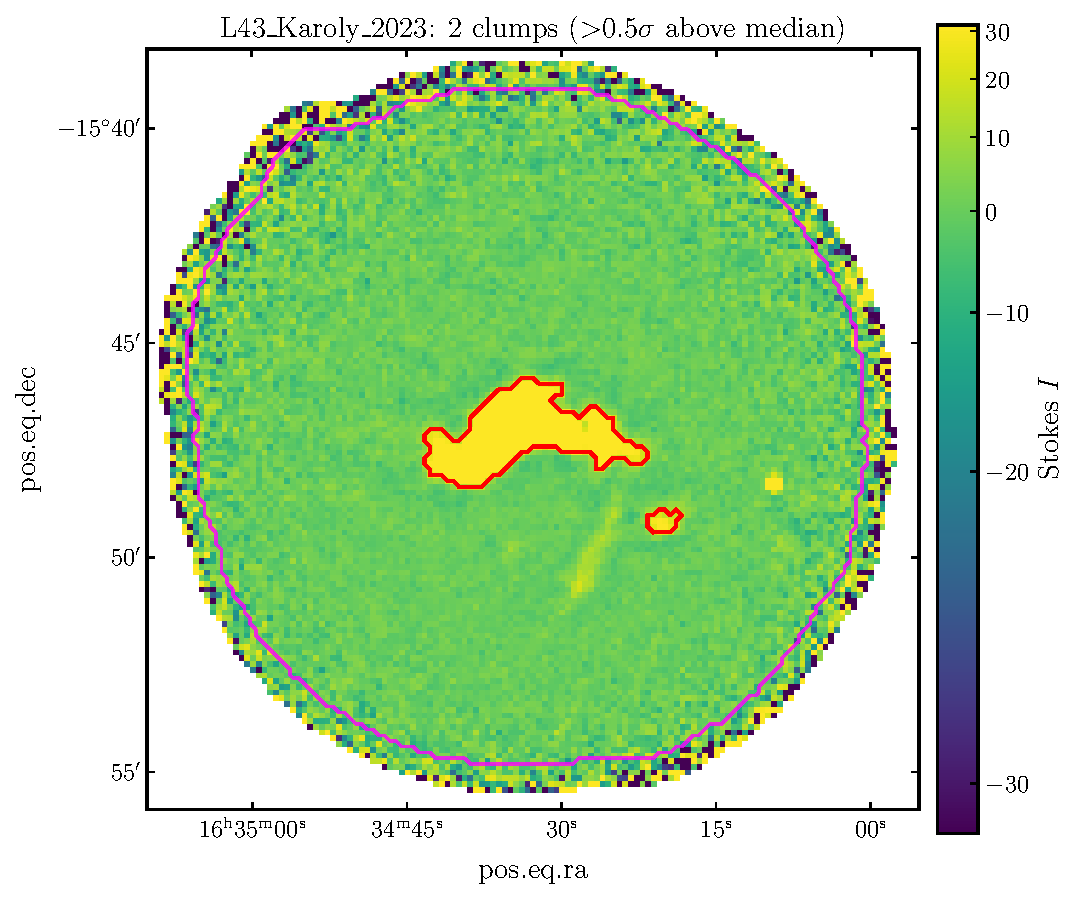
\includegraphics[width=\linewidth]{../plots/L43_Karoly_2023/L43_Karoly_2023_stat_segmentation.pdf}
    \end{subfigure}
    \hfill
    \begin{subfigure}{0.48\textwidth}
        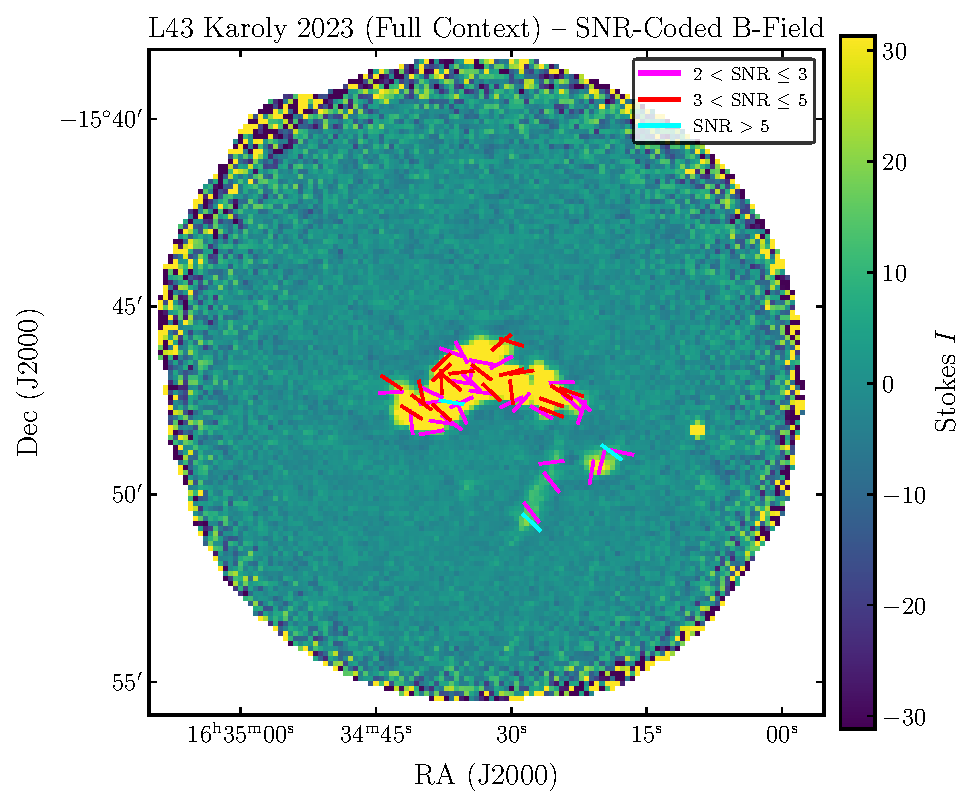
\includegraphics[width=\linewidth]{../plots/L43_Karoly_2023/L43_Karoly_2023_snr_colored_full.pdf}
    \end{subfigure}
    
    \vspace{0.5cm}
    
    \begin{subfigure}{0.6\textwidth}
        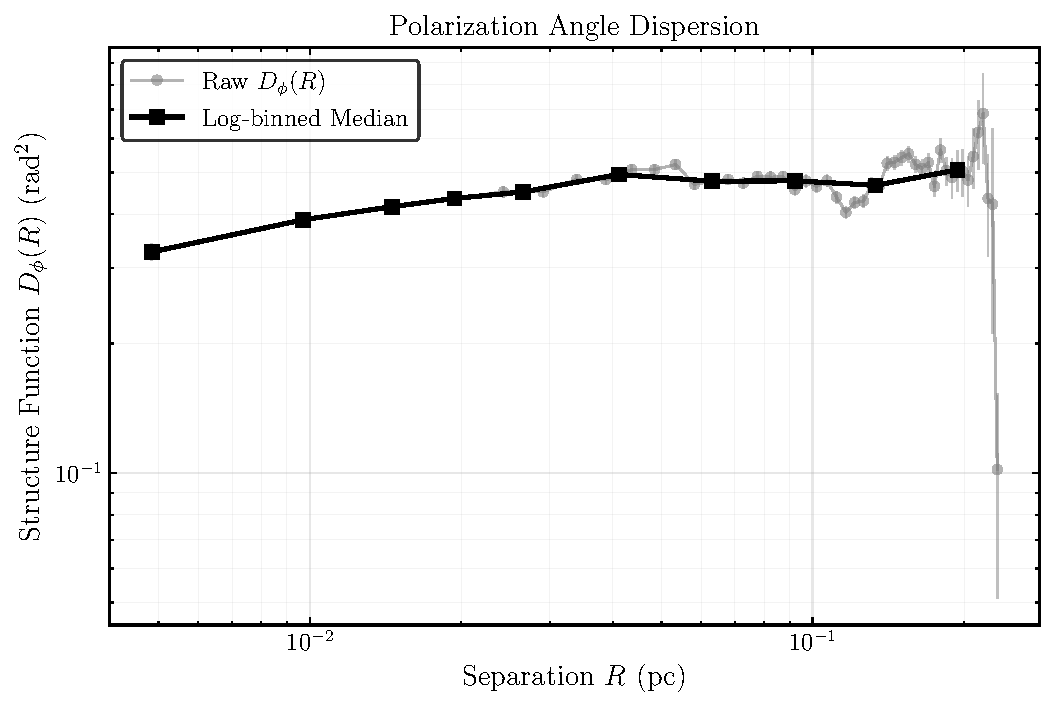
\includegraphics[width=\linewidth]{../plots/L43_Karoly_2023/L43_Karoly_2023_sf.pdf}
    \end{subfigure}
\end{figure}

\newpage
\section*{Target: MonR2}

\begin{table}[H]
    \centering
    \renewcommand{\arraystretch}{1.1}
    \begin{tabular}{ll}
        \toprule
        \textbf{Parameter} & \textbf{Value} \\
        \midrule
        Distance (pc) & 830.0 \\
        Effective Pixels & 3671 \\
        Stokes I RMS & 0.00042 \\
        Median SNR & 1.33 \\
        Distance Reference & Dzib et al. 2016 \\
        Vector Decimation Step & 5 px \\
        \bottomrule
    \end{tabular}
\end{table}

\vspace{0.5cm}

\begin{figure}[H]
    \centering
    \begin{subfigure}{0.48\textwidth}
        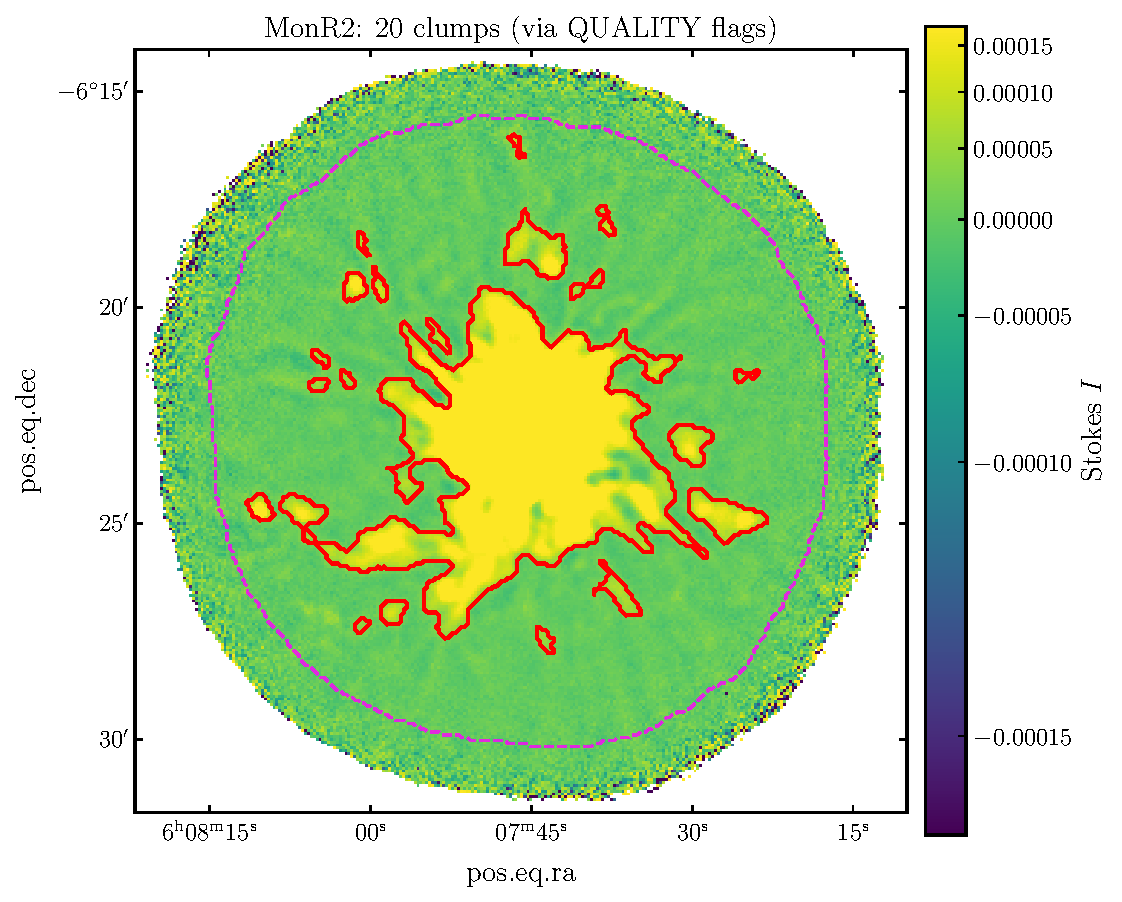
\includegraphics[width=\linewidth]{../plots/MonR2/MonR2_stat_segmentation.pdf}
    \end{subfigure}
    \hfill
    \begin{subfigure}{0.48\textwidth}
        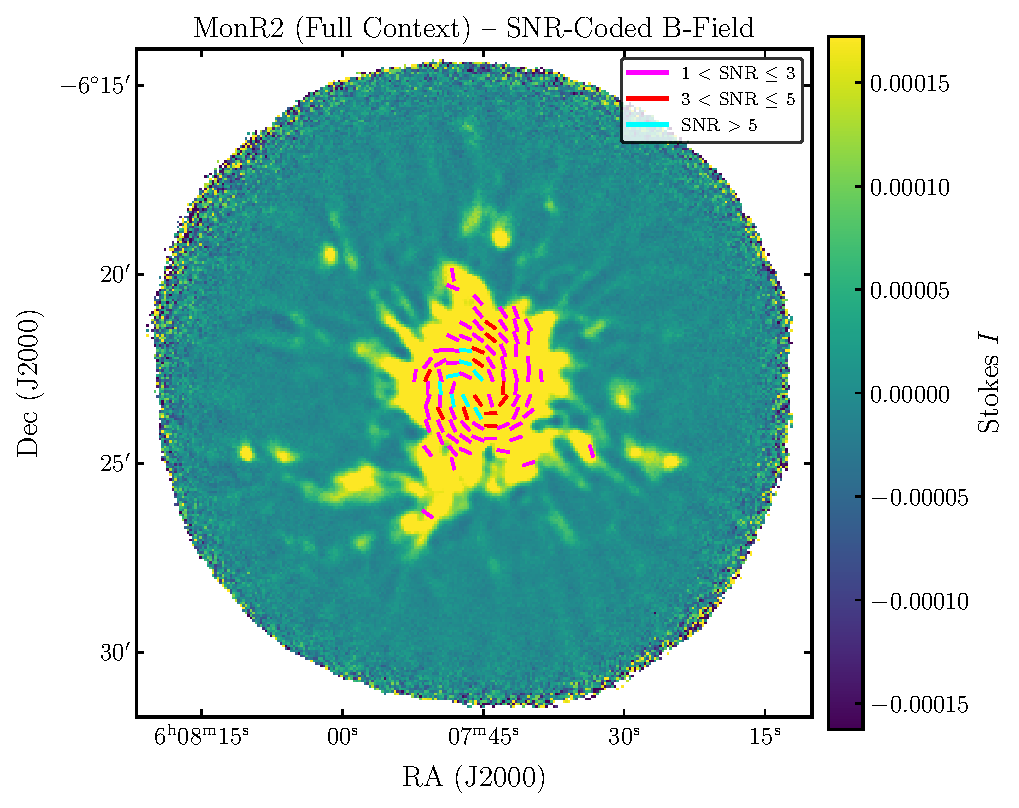
\includegraphics[width=\linewidth]{../plots/MonR2/MonR2_snr_colored_full.pdf}
    \end{subfigure}
    
    \vspace{0.5cm}
    
    \begin{subfigure}{0.6\textwidth}
        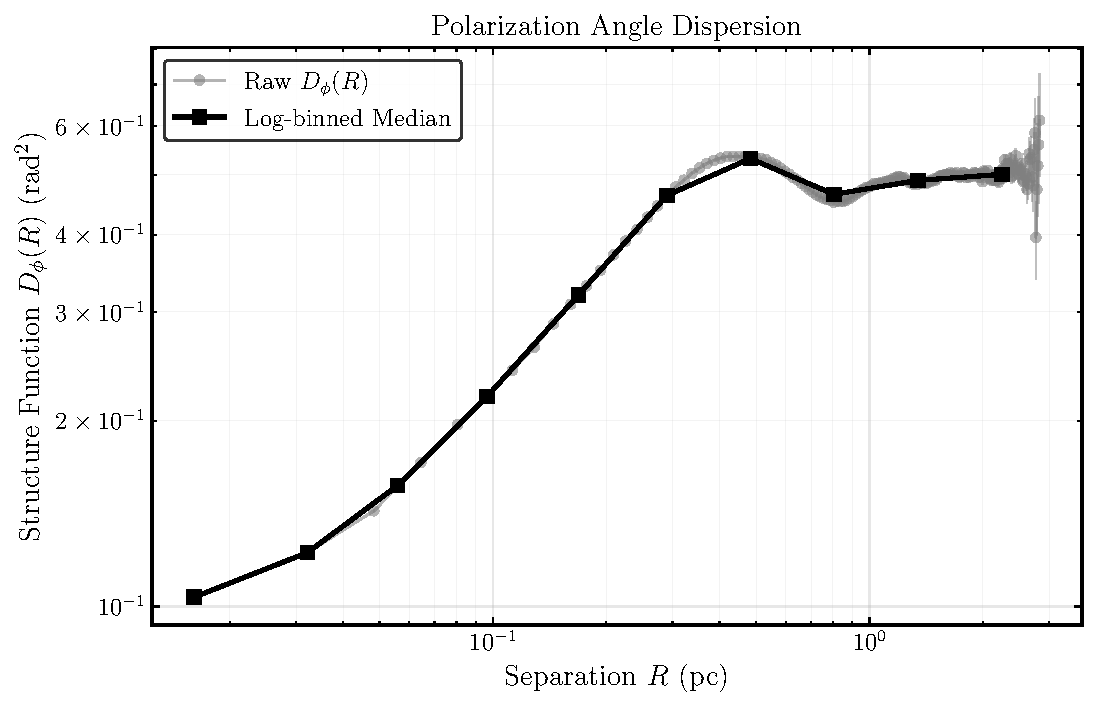
\includegraphics[width=\linewidth]{../plots/MonR2/MonR2_sf.pdf}
    \end{subfigure}
\end{figure}

\newpage
\section*{Target: NGC1333}

\begin{table}[H]
    \centering
    \renewcommand{\arraystretch}{1.1}
    \begin{tabular}{ll}
        \toprule
        \textbf{Parameter} & \textbf{Value} \\
        \midrule
        Distance (pc) & 299.0 \\
        Effective Pixels & 202 \\
        Stokes I RMS & 305.10187 \\
        Median SNR & 2.00 \\
        Distance Reference & Zucker et al. 2018 \\
        Vector Decimation Step & 5 px \\
        \bottomrule
    \end{tabular}
\end{table}

\vspace{0.5cm}

\begin{figure}[H]
    \centering
    \begin{subfigure}{0.48\textwidth}
        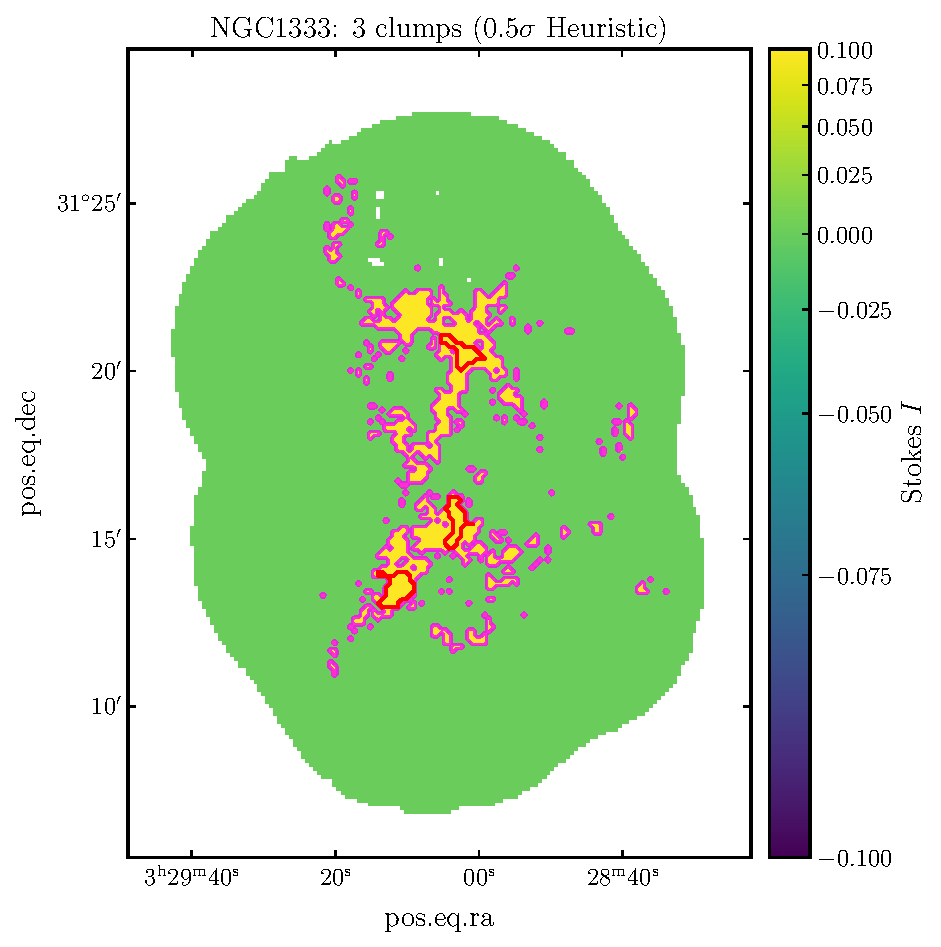
\includegraphics[width=\linewidth]{../plots/NGC1333/NGC1333_stat_segmentation.pdf}
    \end{subfigure}
    \hfill
    \begin{subfigure}{0.48\textwidth}
        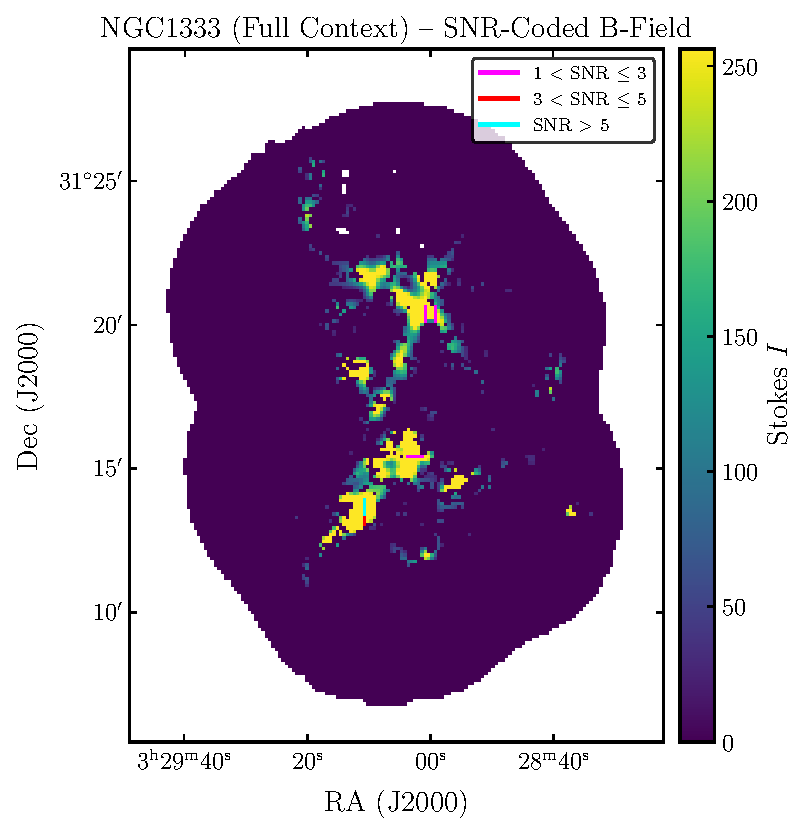
\includegraphics[width=\linewidth]{../plots/NGC1333/NGC1333_snr_colored_full.pdf}
    \end{subfigure}
    
    \vspace{0.5cm}
    
    \begin{subfigure}{0.6\textwidth}
        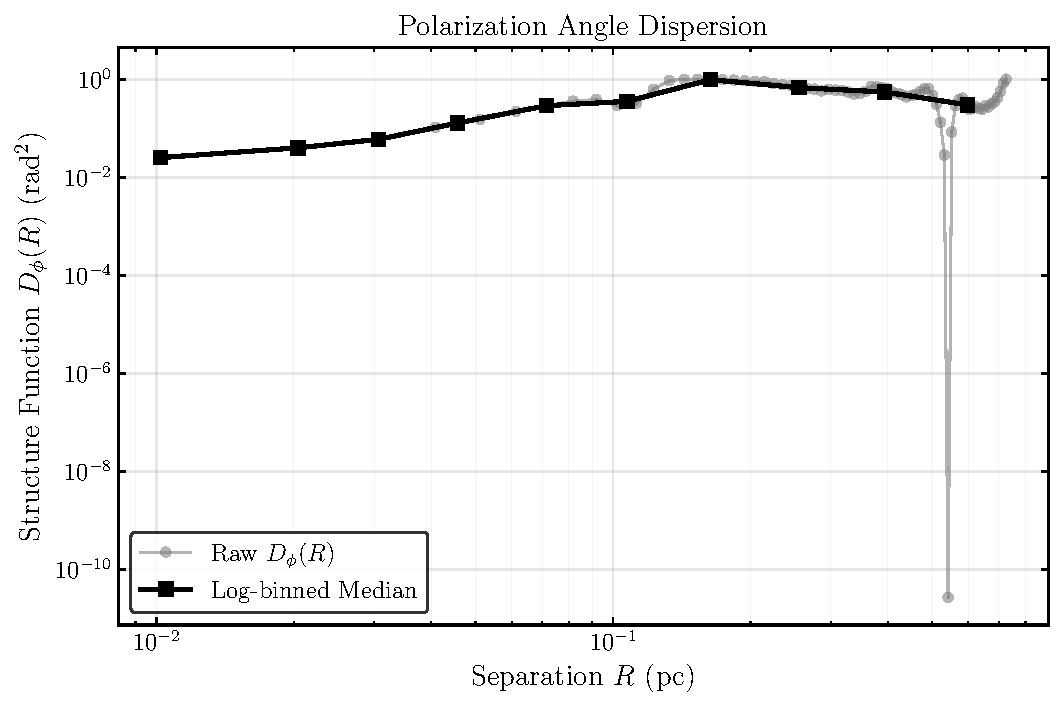
\includegraphics[width=\linewidth]{../plots/NGC1333/NGC1333_sf.pdf}
    \end{subfigure}
\end{figure}

\newpage
\section*{Target: OMC1\_450}

\begin{table}[H]
    \centering
    \renewcommand{\arraystretch}{1.1}
    \begin{tabular}{ll}
        \toprule
        \textbf{Parameter} & \textbf{Value} \\
        \midrule
        Distance (pc) & 388.0 \\
        Effective Pixels & 3841 \\
        Stokes I RMS & 0.00537 \\
        Median SNR & 1.64 \\
        Distance Reference & Kounkel et al. 2017 \\
        Vector Decimation Step & 5 px \\
        \bottomrule
    \end{tabular}
\end{table}

\vspace{0.5cm}

\begin{figure}[H]
    \centering
    \begin{subfigure}{0.48\textwidth}
        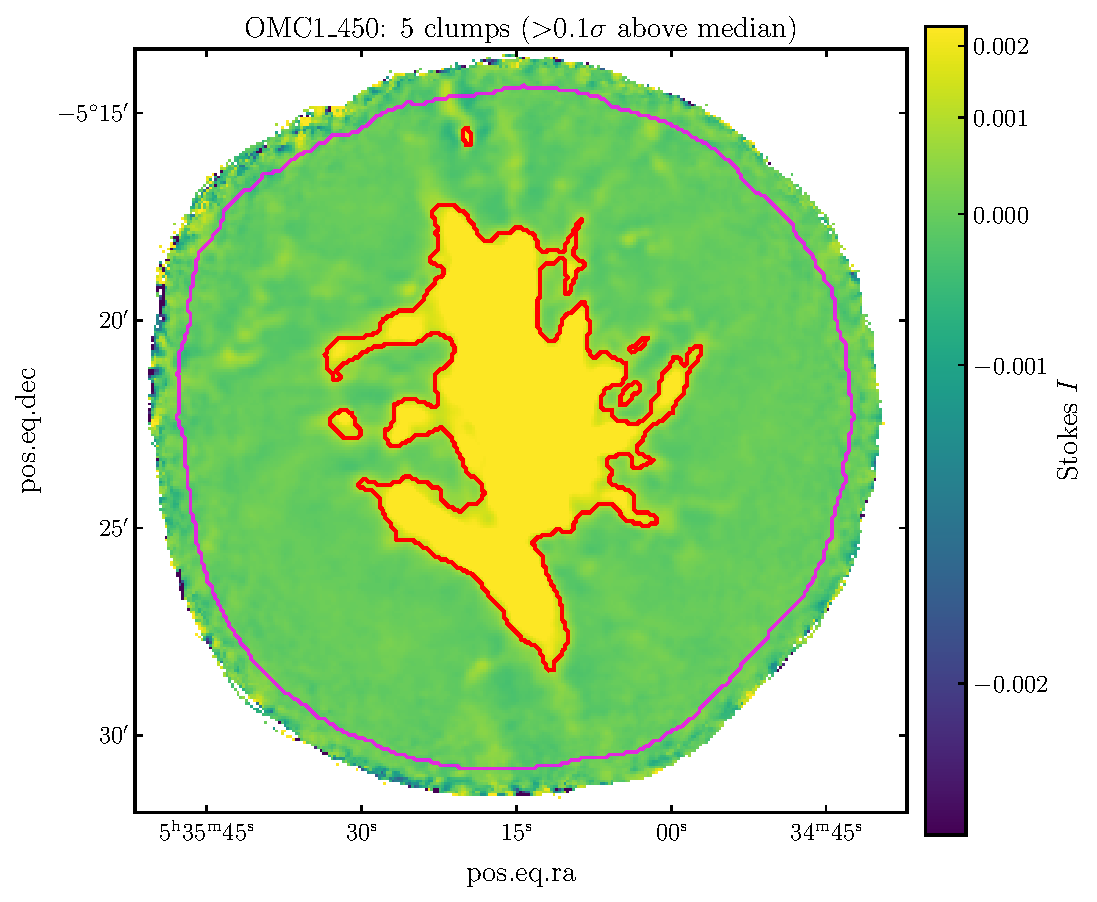
\includegraphics[width=\linewidth]{../plots/OMC1_450/OMC1_450_stat_segmentation.pdf}
    \end{subfigure}
    \hfill
    \begin{subfigure}{0.48\textwidth}
        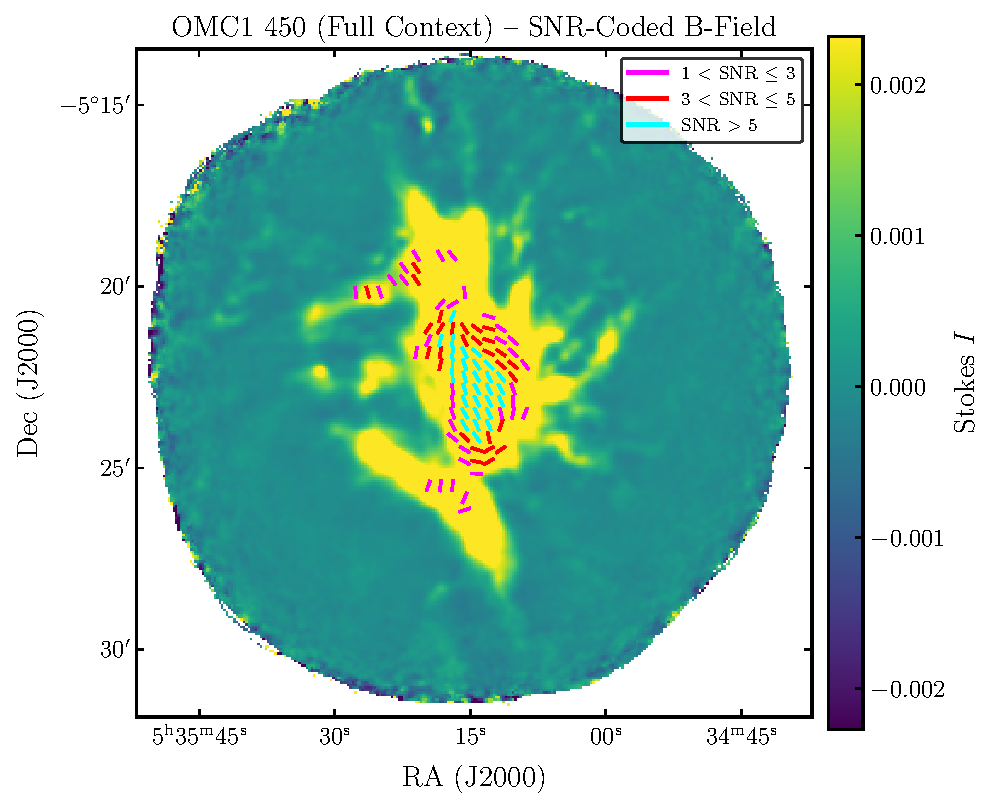
\includegraphics[width=\linewidth]{../plots/OMC1_450/OMC1_450_snr_colored_full.pdf}
    \end{subfigure}
    
    \vspace{0.5cm}
    
    \begin{subfigure}{0.6\textwidth}
        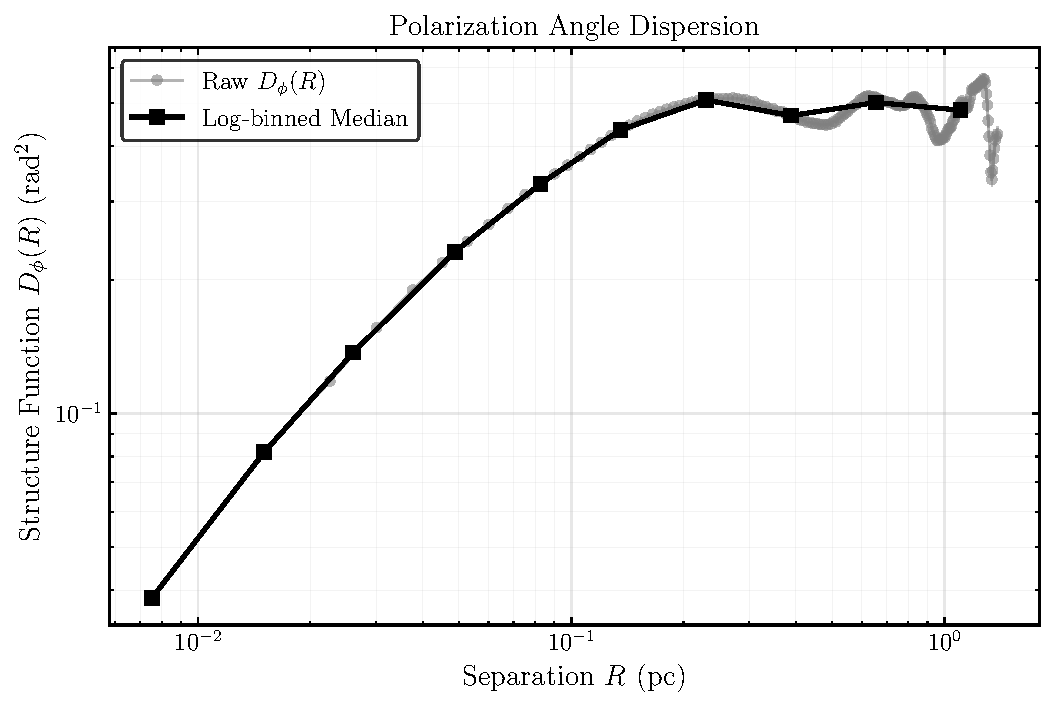
\includegraphics[width=\linewidth]{../plots/OMC1_450/OMC1_450_sf.pdf}
    \end{subfigure}
\end{figure}

\newpage
\section*{Target: OMC1\_850}

\begin{table}[H]
    \centering
    \renewcommand{\arraystretch}{1.1}
    \begin{tabular}{ll}
        \toprule
        \textbf{Parameter} & \textbf{Value} \\
        \midrule
        Distance (pc) & 388.0 \\
        Effective Pixels & 2670 \\
        Stokes I RMS & 0.00226 \\
        Median SNR & 1.72 \\
        Distance Reference & Kounkel et al. 2017 \\
        Vector Decimation Step & 5 px \\
        \bottomrule
    \end{tabular}
\end{table}

\vspace{0.5cm}

\begin{figure}[H]
    \centering
    \begin{subfigure}{0.48\textwidth}
        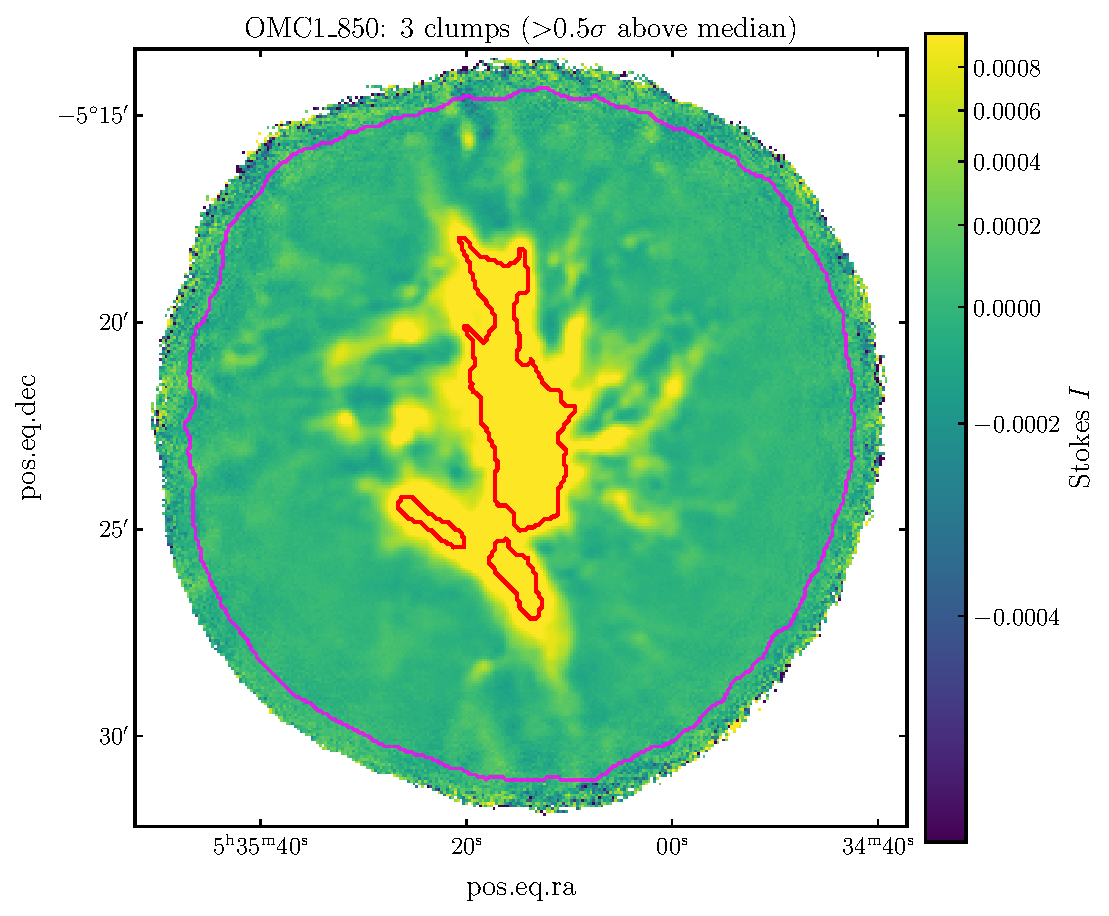
\includegraphics[width=\linewidth]{../plots/OMC1_850/OMC1_850_stat_segmentation.pdf}
    \end{subfigure}
    \hfill
    \begin{subfigure}{0.48\textwidth}
        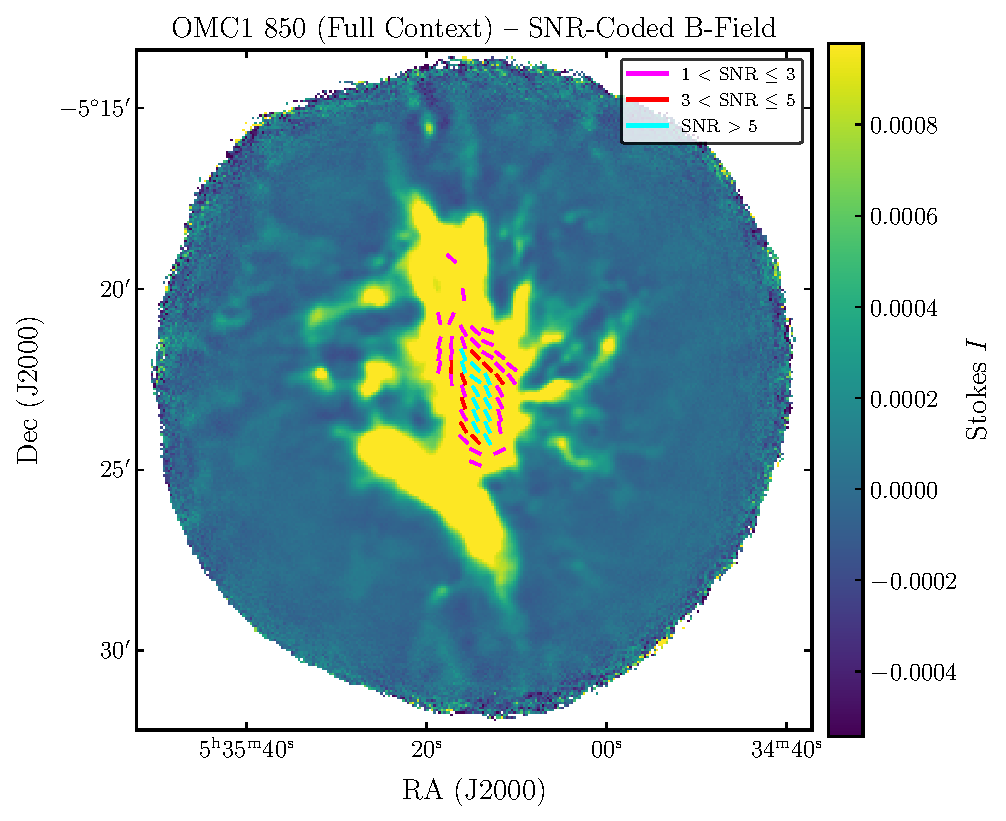
\includegraphics[width=\linewidth]{../plots/OMC1_850/OMC1_850_snr_colored_full.pdf}
    \end{subfigure}
    
    \vspace{0.5cm}
    
    \begin{subfigure}{0.6\textwidth}
        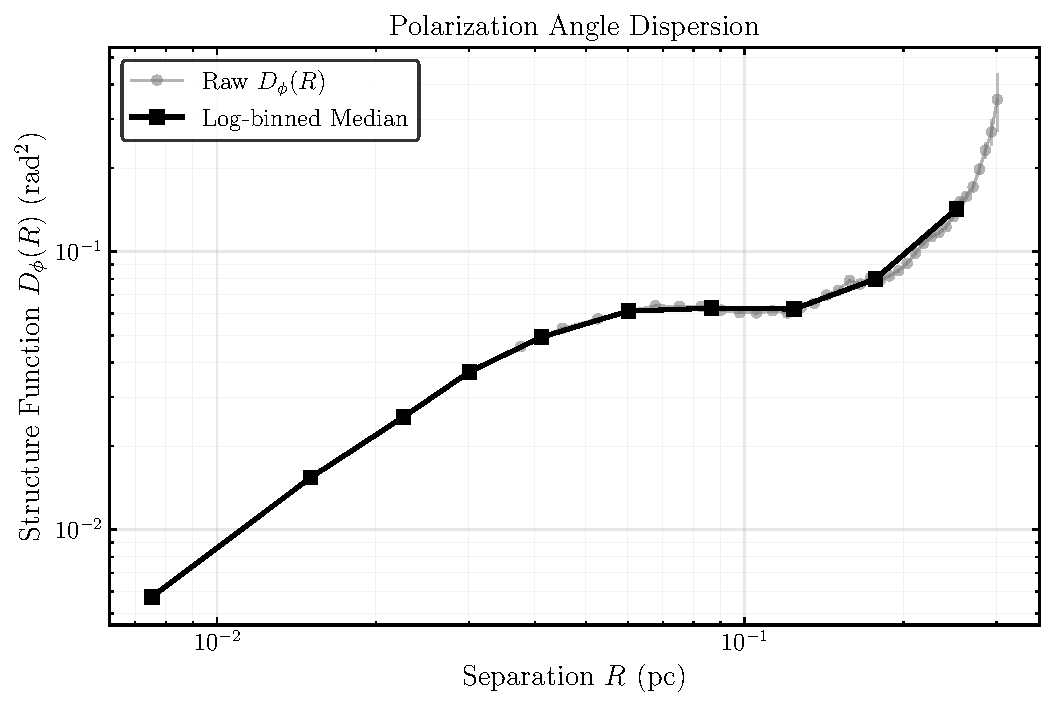
\includegraphics[width=\linewidth]{../plots/OMC1_850/OMC1_850_sf.pdf}
    \end{subfigure}
\end{figure}

\newpage
\section*{Target: Perseus\_B1}

\begin{table}[H]
    \centering
    \renewcommand{\arraystretch}{1.1}
    \begin{tabular}{ll}
        \toprule
        \textbf{Parameter} & \textbf{Value} \\
        \midrule
        Distance (pc) & 293.0 \\
        Effective Pixels & 385 \\
        Stokes I RMS & 0.00006 \\
        Median SNR & 1.49 \\
        Distance Reference & Zucker et al. 2018 \\
        Vector Decimation Step & 3 px \\
        \bottomrule
    \end{tabular}
\end{table}

\vspace{0.5cm}

\begin{figure}[H]
    \centering
    \begin{subfigure}{0.48\textwidth}
        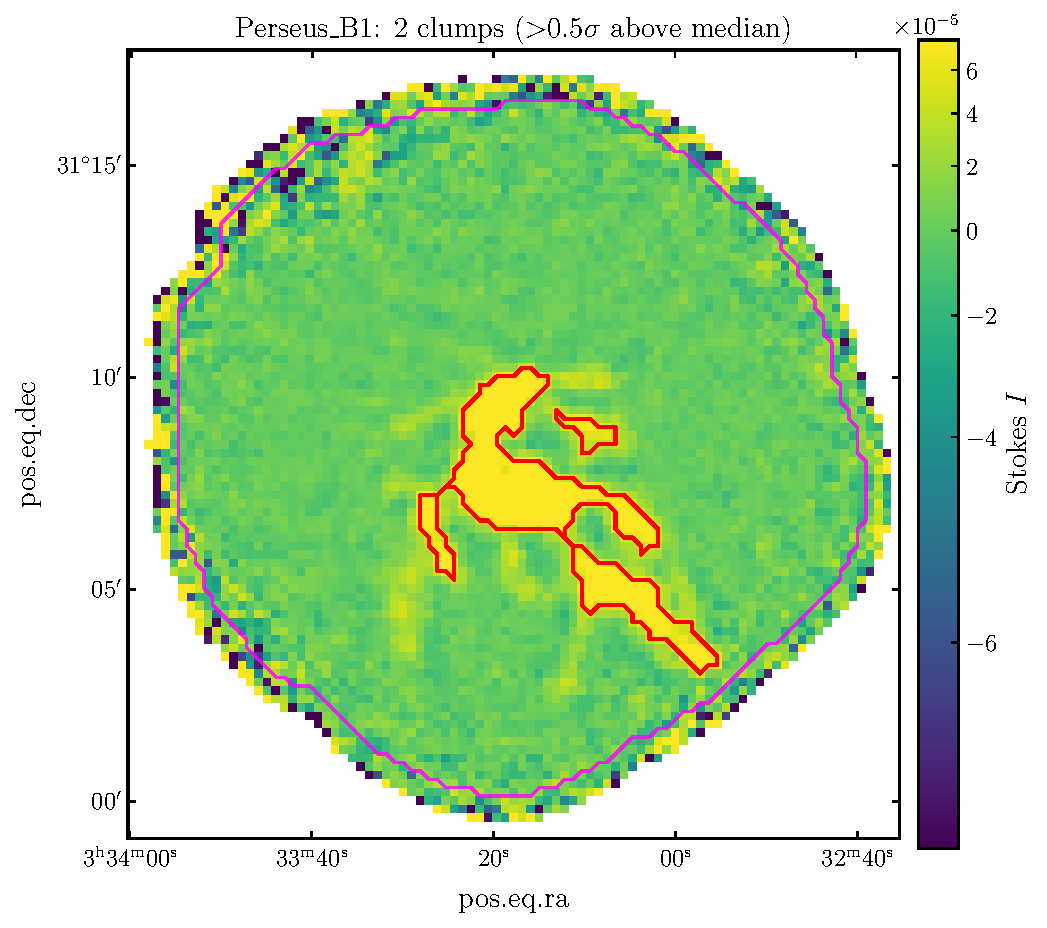
\includegraphics[width=\linewidth]{../plots/Perseus_B1/Perseus_B1_stat_segmentation.pdf}
    \end{subfigure}
    \hfill
    \begin{subfigure}{0.48\textwidth}
        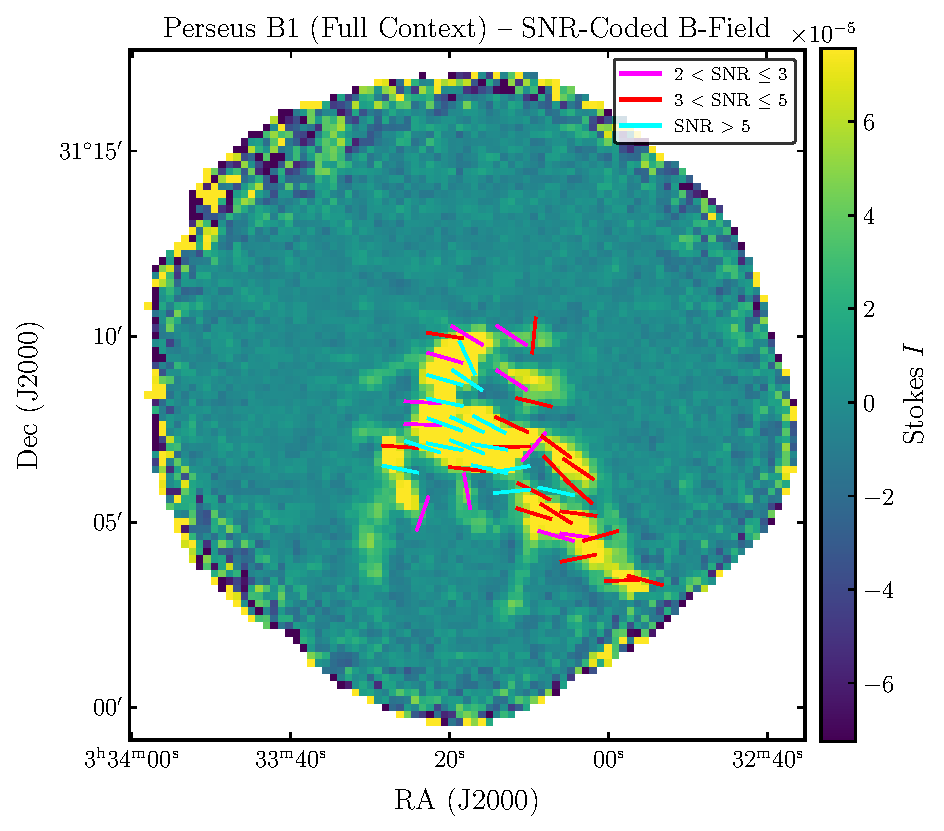
\includegraphics[width=\linewidth]{../plots/Perseus_B1/Perseus_B1_snr_colored_full.pdf}
    \end{subfigure}
    
    \vspace{0.5cm}
    
    \begin{subfigure}{0.6\textwidth}
        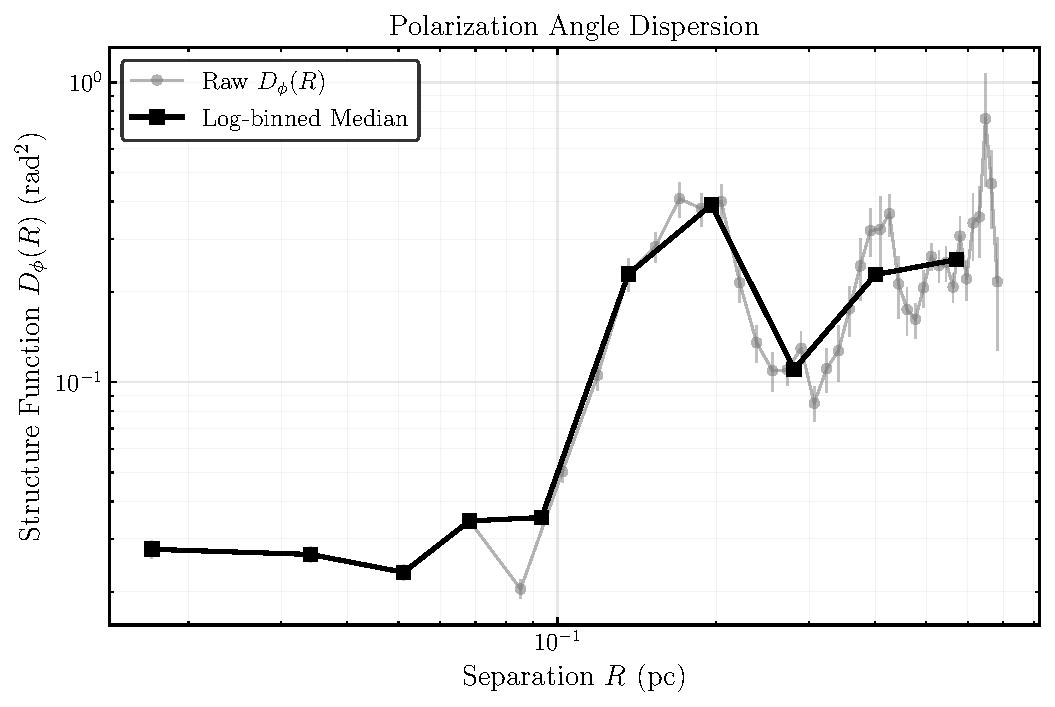
\includegraphics[width=\linewidth]{../plots/Perseus_B1/Perseus_B1_sf.pdf}
    \end{subfigure}
\end{figure}

\newpage
\section*{Target: Rosette}

\begin{table}[H]
    \centering
    \renewcommand{\arraystretch}{1.1}
    \begin{tabular}{ll}
        \toprule
        \textbf{Parameter} & \textbf{Value} \\
        \midrule
        Distance (pc) & 1330.0 \\
        Effective Pixels & 6814 \\
        Stokes I RMS & 25.34009 \\
        Median SNR & 1.37 \\
        Distance Reference & Heyer et al. 2006 \\
        Vector Decimation Step & 6 px \\
        \bottomrule
    \end{tabular}
\end{table}

\vspace{0.5cm}

\begin{figure}[H]
    \centering
    \begin{subfigure}{0.48\textwidth}
        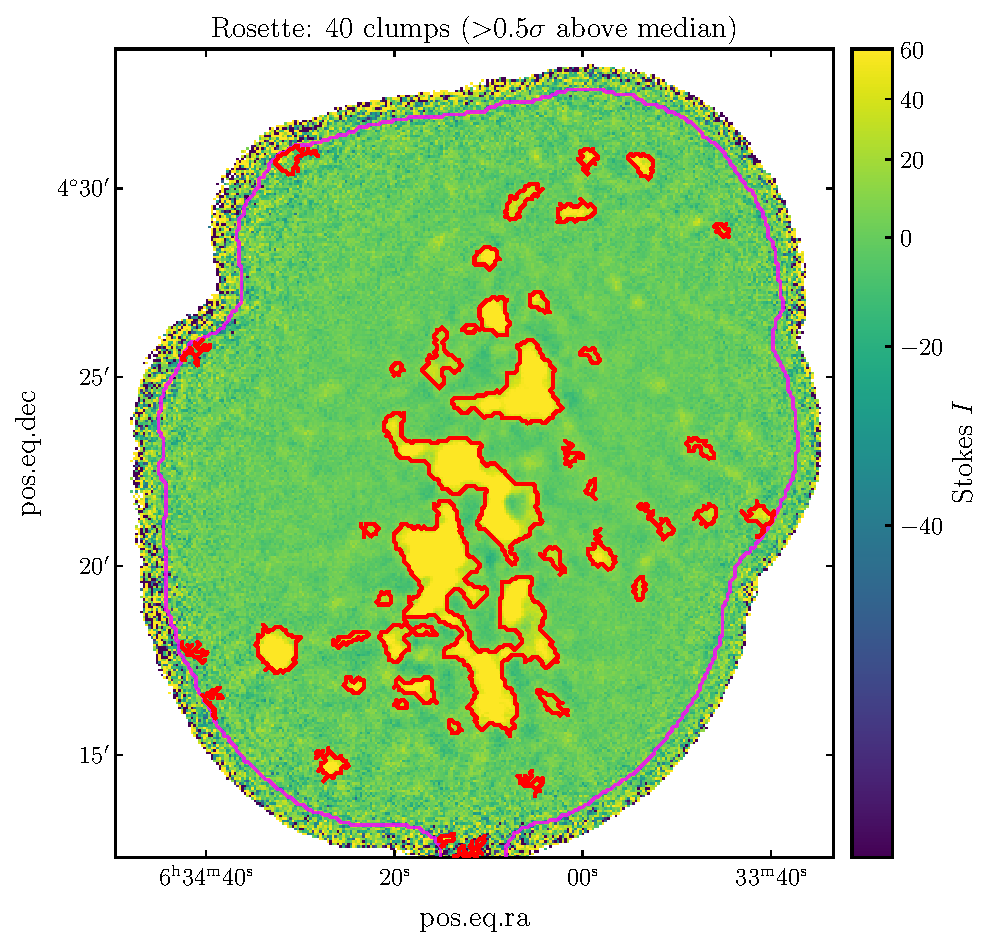
\includegraphics[width=\linewidth]{../plots/Rosette/Rosette_stat_segmentation.pdf}
    \end{subfigure}
    \hfill
    \begin{subfigure}{0.48\textwidth}
        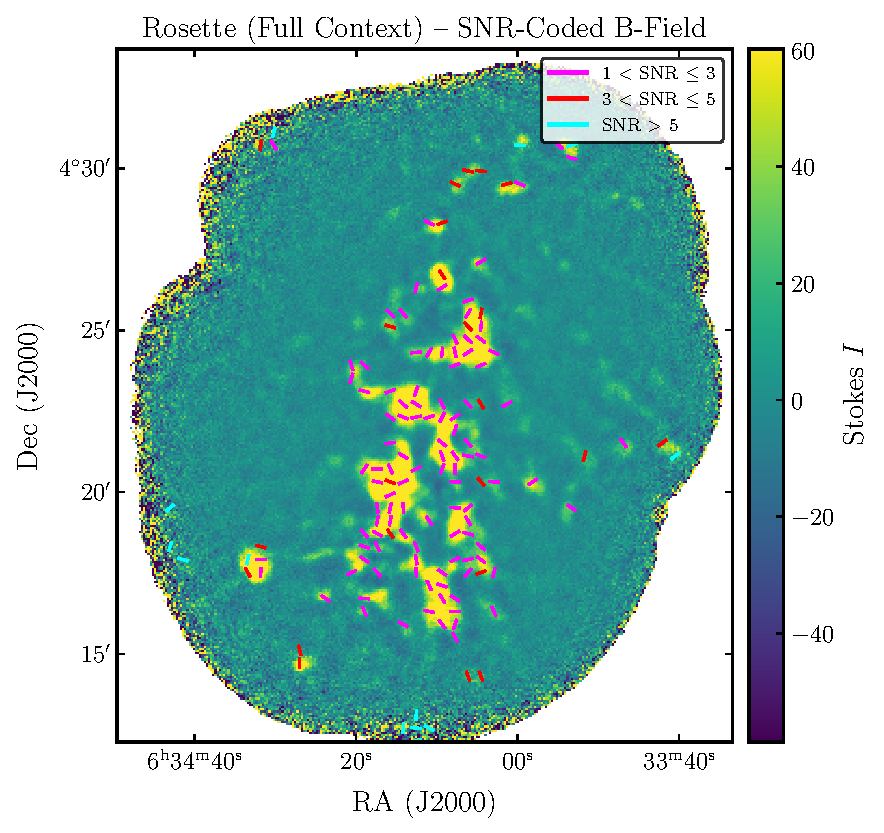
\includegraphics[width=\linewidth]{../plots/Rosette/Rosette_snr_colored_full.pdf}
    \end{subfigure}
    
    \vspace{0.5cm}
    
    \begin{subfigure}{0.6\textwidth}
        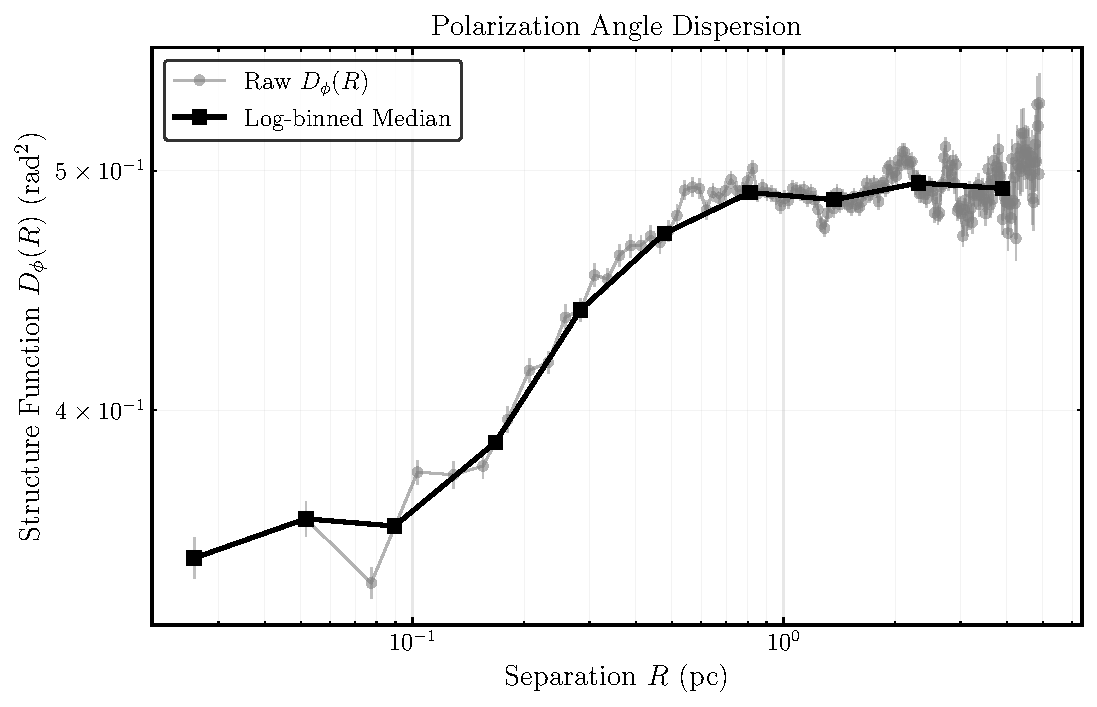
\includegraphics[width=\linewidth]{../plots/Rosette/Rosette_sf.pdf}
    \end{subfigure}
\end{figure}

\newpage
\section*{Target: oph\_a}

\begin{table}[H]
    \centering
    \renewcommand{\arraystretch}{1.1}
    \begin{tabular}{ll}
        \toprule
        \textbf{Parameter} & \textbf{Value} \\
        \midrule
        Distance (pc) & 139.0 \\
        Effective Pixels & 2135 \\
        Stokes I RMS & 185.76798 \\
        Median SNR & 1.27 \\
        Distance Reference & Zucker et al. 2019 \\
        Vector Decimation Step & 6 px \\
        \bottomrule
    \end{tabular}
\end{table}

\vspace{0.5cm}

\begin{figure}[H]
    \centering
    \begin{subfigure}{0.48\textwidth}
        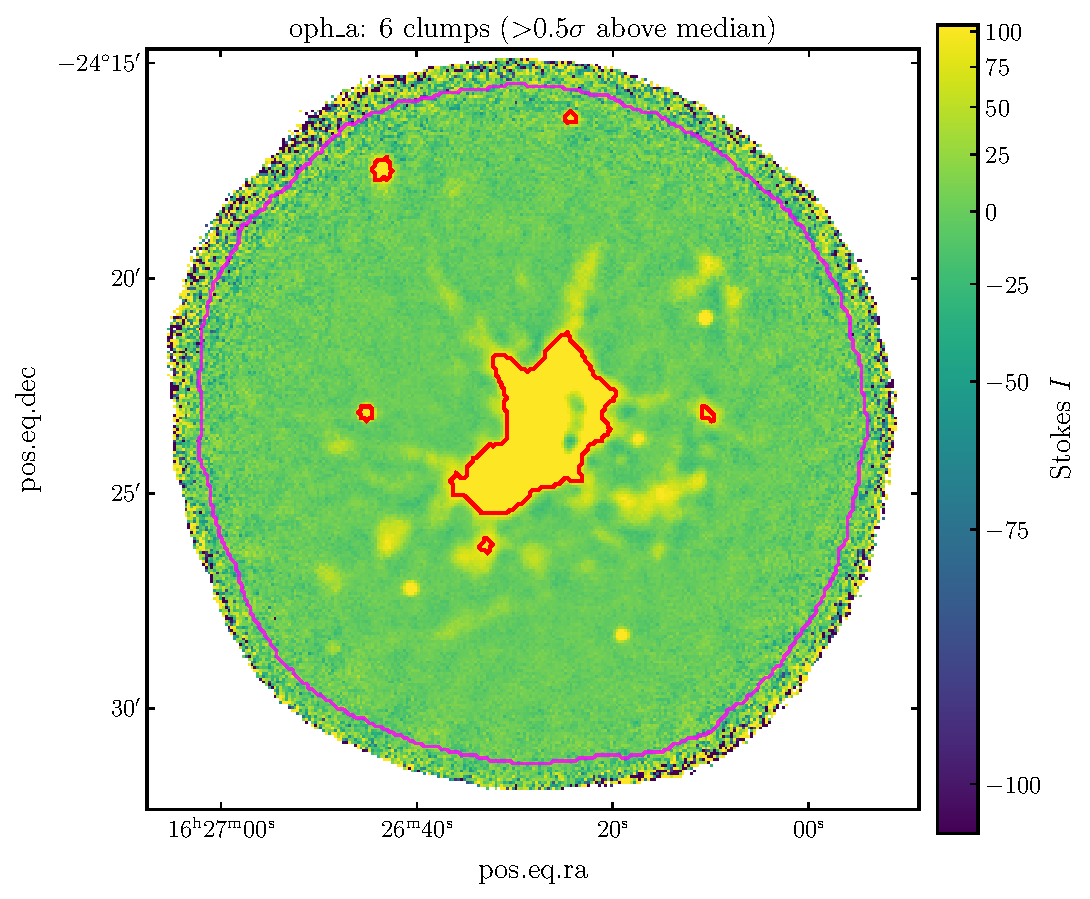
\includegraphics[width=\linewidth]{../plots/oph_a/oph_a_stat_segmentation.pdf}
    \end{subfigure}
    \hfill
    \begin{subfigure}{0.48\textwidth}
        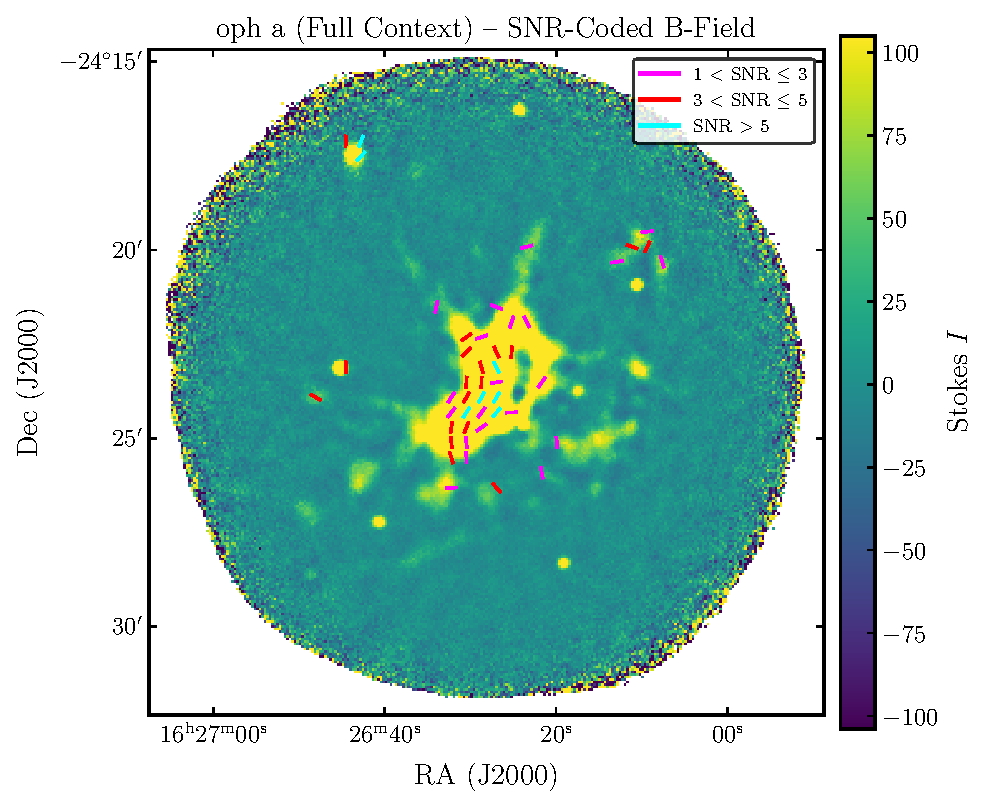
\includegraphics[width=\linewidth]{../plots/oph_a/oph_a_snr_colored_full.pdf}
    \end{subfigure}
    
    \vspace{0.5cm}
    
    \begin{subfigure}{0.6\textwidth}
        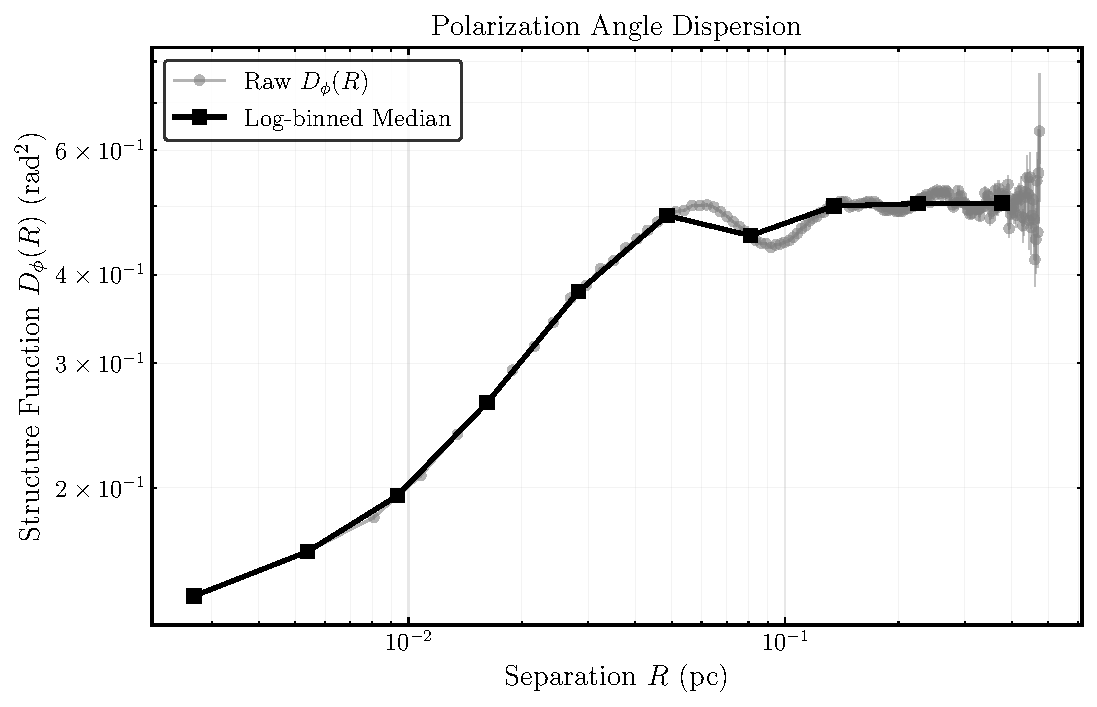
\includegraphics[width=\linewidth]{../plots/oph_a/oph_a_sf.pdf}
    \end{subfigure}
\end{figure}

\newpage
\section*{Target: oph\_b}

\begin{table}[H]
    \centering
    \renewcommand{\arraystretch}{1.1}
    \begin{tabular}{ll}
        \toprule
        \textbf{Parameter} & \textbf{Value} \\
        \midrule
        Distance (pc) & 139.0 \\
        Effective Pixels & 3503 \\
        Stokes I RMS & 85.63193 \\
        Median SNR & 1.16 \\
        Distance Reference & Zucker et al. 2019 \\
        Vector Decimation Step & 6 px \\
        \bottomrule
    \end{tabular}
\end{table}

\vspace{0.5cm}

\begin{figure}[H]
    \centering
    \begin{subfigure}{0.48\textwidth}
        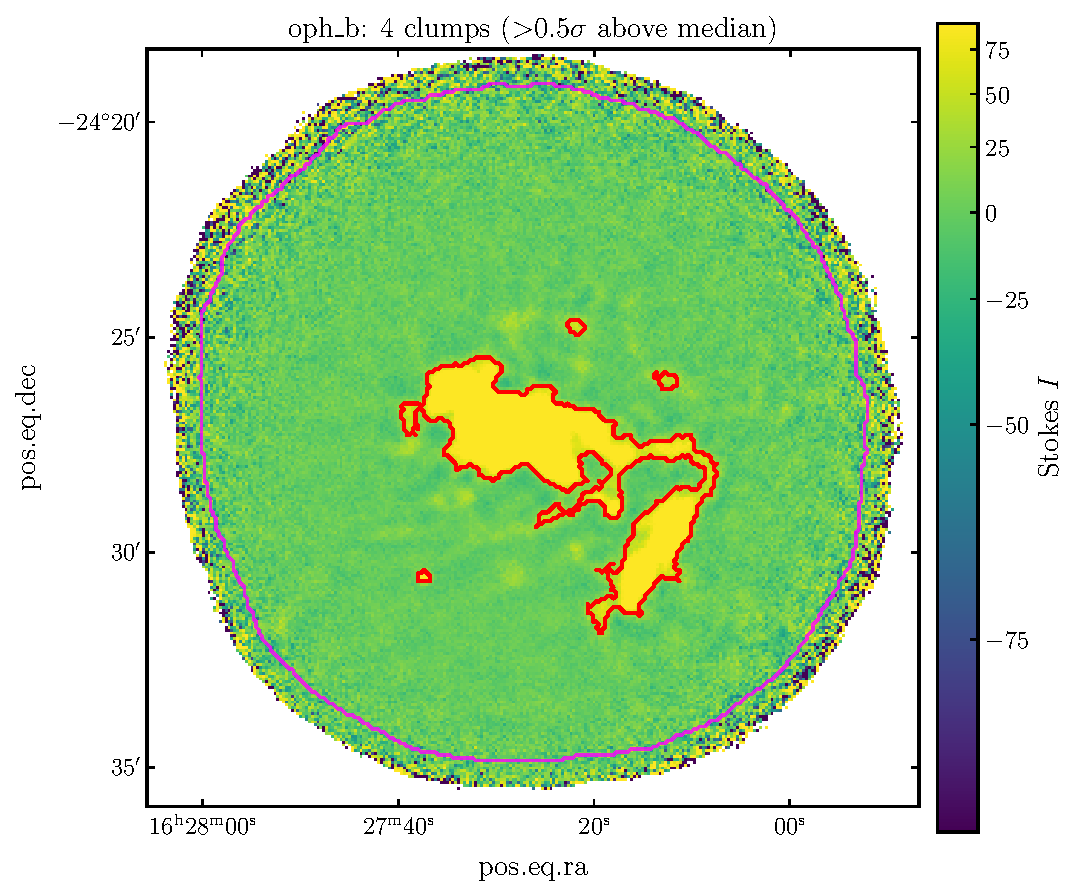
\includegraphics[width=\linewidth]{../plots/oph_b/oph_b_stat_segmentation.pdf}
    \end{subfigure}
    \hfill
    \begin{subfigure}{0.48\textwidth}
        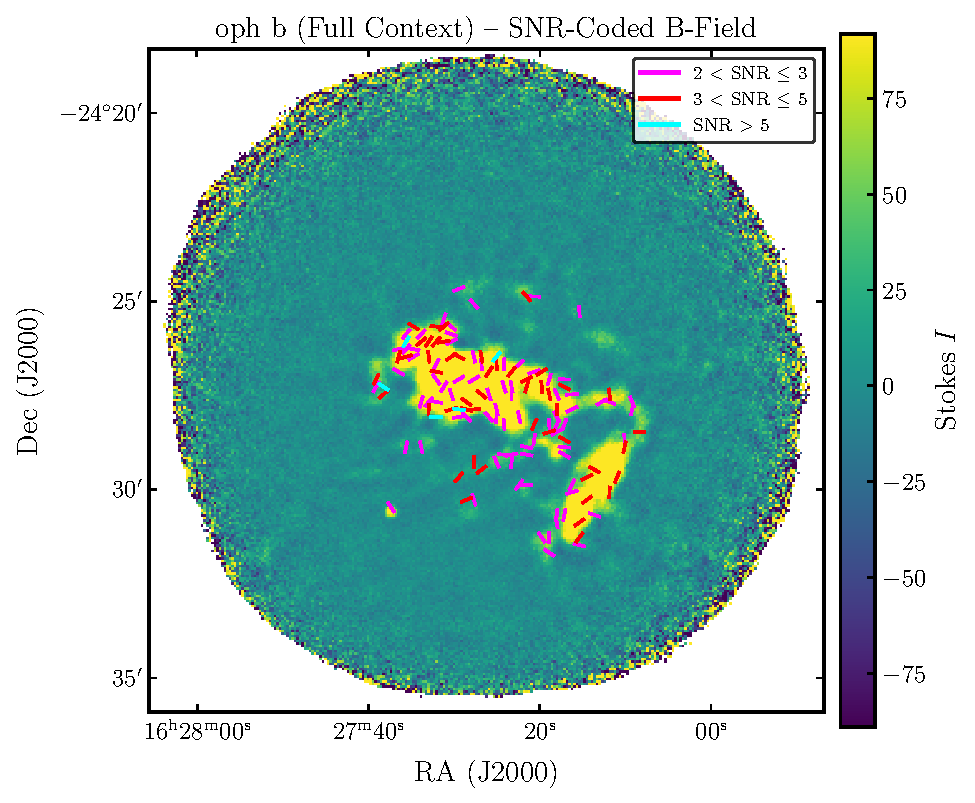
\includegraphics[width=\linewidth]{../plots/oph_b/oph_b_snr_colored_full.pdf}
    \end{subfigure}
    
    \vspace{0.5cm}
    
    \begin{subfigure}{0.6\textwidth}
        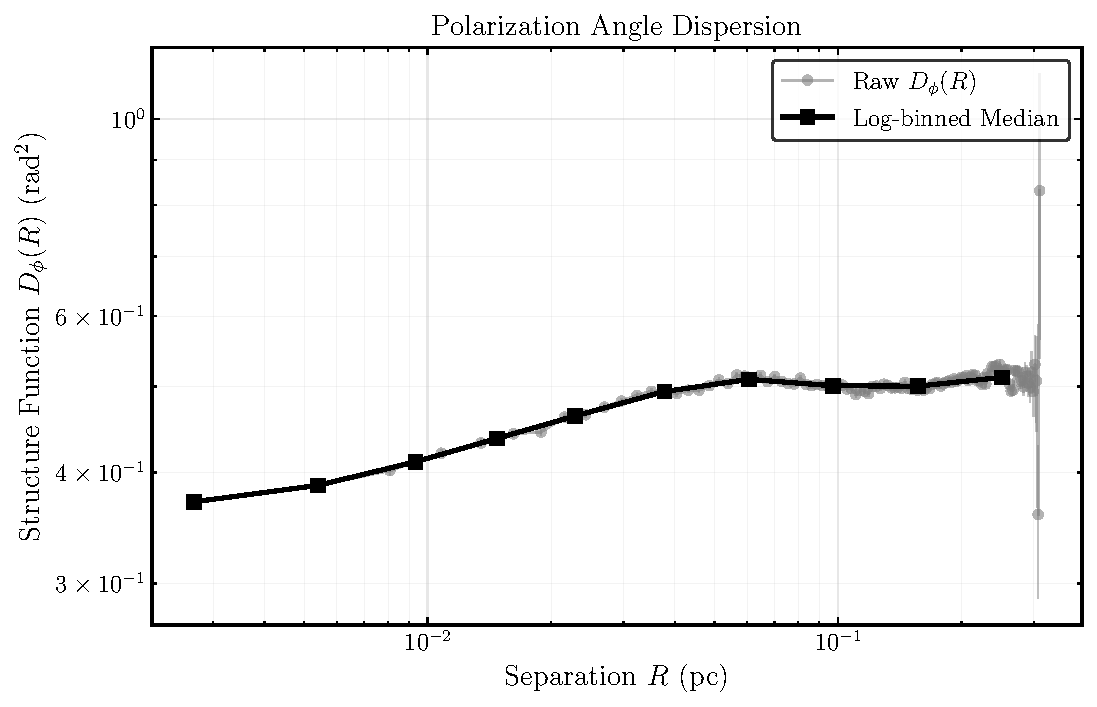
\includegraphics[width=\linewidth]{../plots/oph_b/oph_b_sf.pdf}
    \end{subfigure}
\end{figure}

\newpage
\section*{Target: oph\_c}

\begin{table}[H]
    \centering
    \renewcommand{\arraystretch}{1.1}
    \begin{tabular}{ll}
        \toprule
        \textbf{Parameter} & \textbf{Value} \\
        \midrule
        Distance (pc) & 139.0 \\
        Effective Pixels & 4145 \\
        Stokes I RMS & 33.63853 \\
        Median SNR & 1.34 \\
        Distance Reference & Zucker et al. 2019 \\
        Vector Decimation Step & 6 px \\
        \bottomrule
    \end{tabular}
\end{table}

\vspace{0.5cm}

\begin{figure}[H]
    \centering
    \begin{subfigure}{0.48\textwidth}
        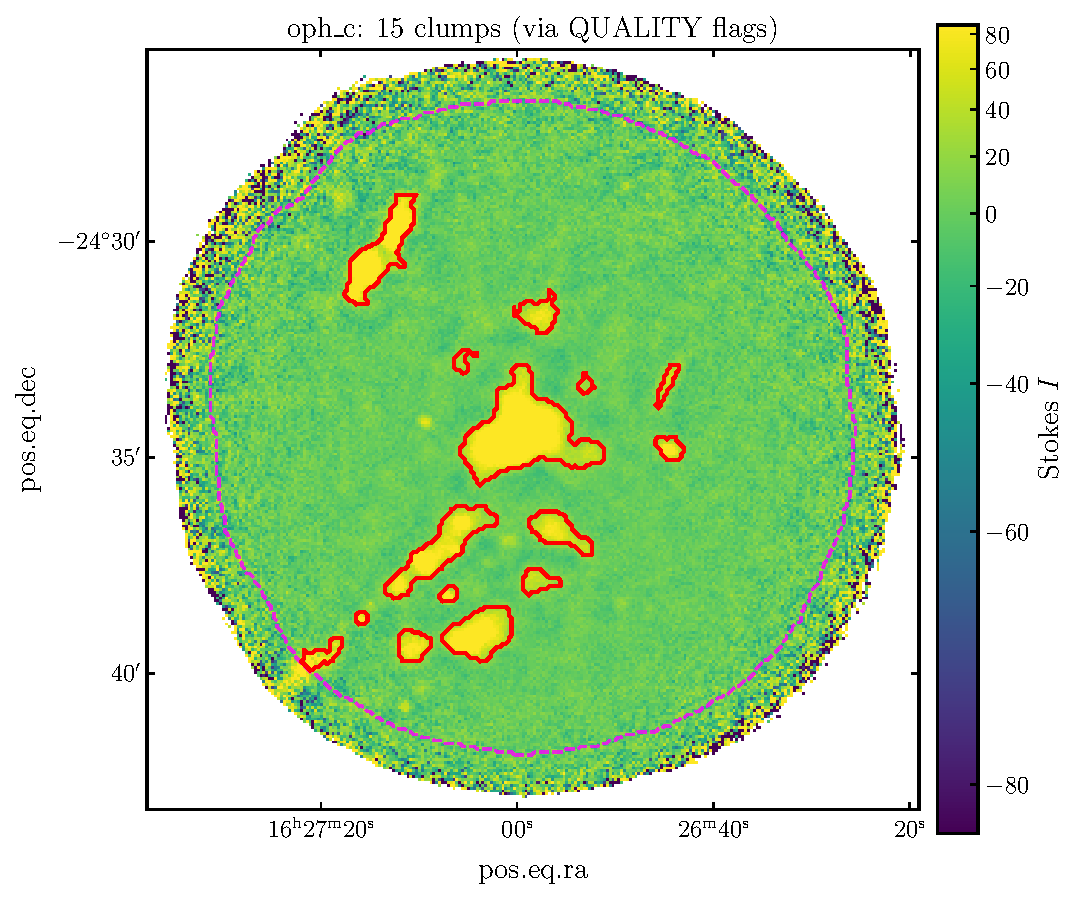
\includegraphics[width=\linewidth]{../plots/oph_c/oph_c_stat_segmentation.pdf}
    \end{subfigure}
    \hfill
    \begin{subfigure}{0.48\textwidth}
        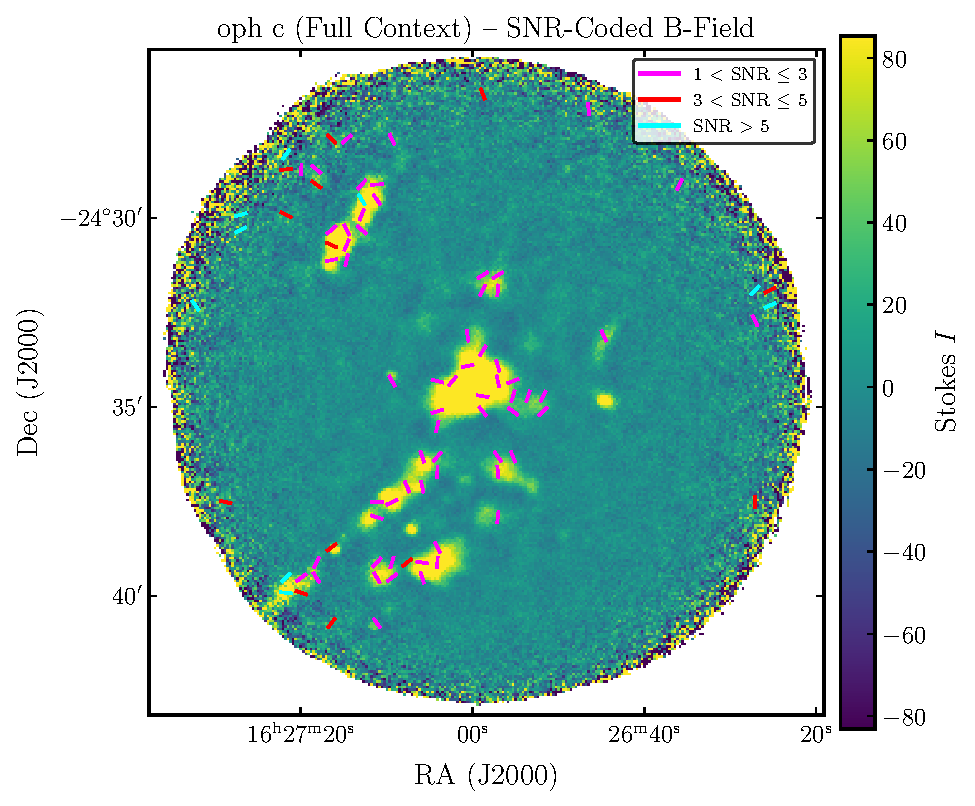
\includegraphics[width=\linewidth]{../plots/oph_c/oph_c_snr_colored_full.pdf}
    \end{subfigure}
    
    \vspace{0.5cm}
    
    \begin{subfigure}{0.6\textwidth}
        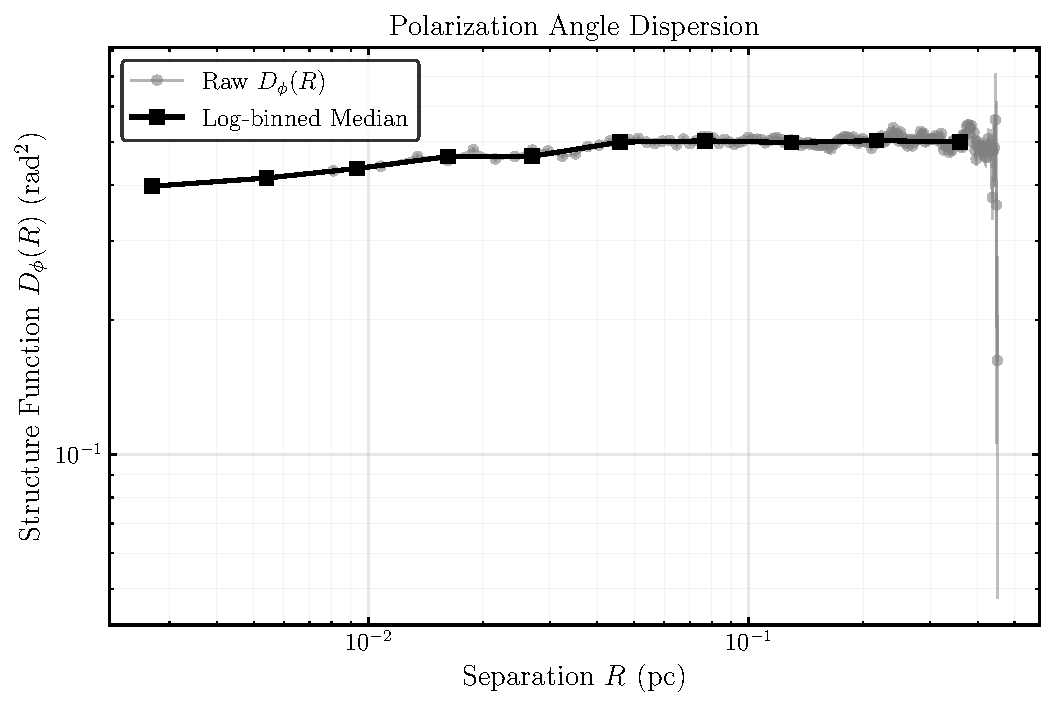
\includegraphics[width=\linewidth]{../plots/oph_c/oph_c_sf.pdf}
    \end{subfigure}
\end{figure}

\newpage
\end{document}